\documentclass[a4paper,fleqn]{cas-dc}
\hypersetup{hypertexnames=false}
\usepackage[sort,numbers]{natbib}
\usepackage{amsmath}
\usepackage{amssymb}
\usepackage{amsthm}
\usepackage{algorithm}
\usepackage[commentColor=black,beginComment=//~,endComment={},beginLComment=//~,endLComment={},italicComments=false]{algpseudocodex}
\tikzset{algpxIndentLine/.style={draw=black}}
\algrenewcommand{\alglinenumber}[1]{\bfseries\footnotesize #1}
\algrenewcommand{\textproc}{}
\algrenewcommand{\algorithmicrequire}{\textbf{Input:}}
\algrenewcommand{\algorithmicensure}{\textbf{Output:}}
\newtheorem{theorem}{Theorem}
\newtheorem{proposition}{Proposition}
\newcommand{\method}{\textsc{FedGauss}}
\newcommand{\MethodinCaption}{F\raisebox{-0.05ex}{\scalebox{0.80}{ED}}G\raisebox{-0.05ex}{\scalebox{0.80}{AUSS}}}
\usepackage{xcolor}
\usepackage{tabularray}
\usepackage{ragged2e}
\setcounter{totalnumber}{9}
\setcounter{topnumber}{9}
\setcounter{bottomnumber}{9}
\setcounter{dbltopnumber}{9}
\renewcommand{\topfraction}{.95}
\renewcommand{\dbltopfraction}{.95}
\renewcommand{\bottomfraction}{.05}
\renewcommand{\textfraction}{.05}
\renewcommand{\floatpagefraction}{.95}
\renewcommand{\dblfloatpagefraction}{.95}
\usepackage[caption=false,font=footnotesize]{subfig}
\captionsetup[subfloat]{subrefformat=simple,labelformat=simple}
\renewcommand{\thesubfigure}{(\alph{subfigure})}
\usepackage[nameinlink]{cleveref}
\crefname{theorem}{Theorem}{Theorems}
\crefname{proposition}{Proposition}{Propositions}
\crefname{figure}{\figurename}{\figurename s}
\crefname{table}{\tablename}{\tablename s}
\crefname{section}{Section}{Sections}
\crefname{algorithm}{Algorithm}{Algorithms}
\begin{document}
\shorttitle{}
\shortauthors{diyigezuozhemingzi et~al.}
\title[mode=title]{FedGauss: Federated Gaussian-noise Release under Transcript-Conditioned Accounting}
\tnotemark[1]
\tnotetext[1]{This document is the results of the research project funded by the National Science Foundation.}
\author[1]{Author One}[orcid=0000-0001-0000-0000]
\ead{1111@example.in}
\author[2]{Author Two}[orcid=0000-0001-0000-0000]
\cormark[1]
\ead{222@example.in}
\author[1,3]{Author Three}[orcid=0000-0001-0000-0000]
\ead{333@example.in}
\author[1,3]{Author Four}[orcid=0000-0001-0000-0000]
\ead{444@example.in}
\affiliation[1]{organization={Department of Physics, J.K. Institute of Science},
addressline={Jawahar Nagar},
city={Trivandrum},
postcode={695013},
state={Kerala},
country={India}}
\affiliation[2]{organization={Department of Physics, J.K. Institute of Science},
addressline={Jawahar Nagar},
city={Trivandrum},
postcode={695013},
state={Kerala},
country={India}}
\affiliation[3]{organization={Department of Physics, J.K. Institute of Science},
addressline={Jawahar Nagar},
city={Trivandrum},
postcode={695013},
state={Kerala},
country={India}}
\cortext[cor1]{Corresponding author}
\begin{abstract}
Edge intrusion detection requires a model that adapts to each client's local traffic distribution, yet raw traffic records cannot be uploaded centrally. Federated LoRA supports this adaptation by aggregating client adapter updates instead of raw data. Adapter updates, however, still encode client-specific traffic patterns, so client-level differential privacy (DP) is typically required. DP is meant to exchange a bounded utility loss for this protection. Deployed in its common per-client form, it instead appears to collapse the detection utility of federated LoRA. This paper asks where the privacy cost of DP-protected federated LoRA actually comes from. We decompose the gap over four candidate design choices, namely the release boundary, the accounting configuration, the clipping calibration, and the representation space. We answer with \method, a two-branch release protocol evaluated as a matched factorial under a common transcript-aware privacy-accounting framework and one total budget on three intrusion-detection benchmarks. The four factors are exposed as controlled variables rather than confounded. The evaluation yields three findings. First, most of the privacy cost is an accounting-and-clipping artifact, since tight accounting and a tuned clip let the same per-client release recover most of its utility loss, for example, from 0.4533 to 0.8014 Macro-F1 on UNSW-NB15. Second, part of the cost is a joint effect of the release boundary and the representation space, and this margin is modest and dimension-dependent. Third, basis provenance contributes nothing, because public and seeded random bases are indistinguishable in every protocol-matched comparison.
\end{abstract}
\begin{keywords}
Federated learning \sep Federated LoRA \sep Differential privacy \sep Privacy--utility attribution \sep Network intrusion detection
\end{keywords}
\begin{NoHyper}
\maketitle
\end{NoHyper}
\section{Introduction}
\label{sec:introduction}
\par
Pre-trained models are increasingly deployed at the network edge to support IoT analytics, encrypted traffic classification, and intrusion detection. In network-security operations, edge gateways and monitoring nodes must adapt traffic or event classifiers to local device populations, attack patterns, and protocol distributions, without exposing raw packet traces or security logs~\cite{qu2025mobileedge}. Centralizing such adaptation is not an option, because raw traffic and security logs cannot be shipped off the devices that generate them. Edge devices likewise cannot afford to train or exchange full model weights on their own. Federated learning (FL) supplies the training paradigm for this setting~\cite{mcmahan2017communication,li2020federated}, and low-rank adaptation (LoRA) makes it practical at the edge by having clients exchange compact adapter states instead of full model
weights~\cite{hu2022lora,sun2024ffalora,singhal2025fedexlora}.
Adapter updates, although compact, remain data-dependent. They encode client-specific traffic patterns and membership signals, and inversion attacks tailored to adapter-style fine-tuning can reconstruct user data from them~\cite{sami2025adapter}. Client-level differential privacy (DP) is
therefore the standard defense~\cite{dwork2014algorithmic,abadi2016deep}, yet in its per-client form, with each upload Gaussian-sanitized under basic composition and a conservative clip, DP appears to make protected federated LoRA unusable, and conventional per-client configurations can substantially reduce detection utility. This raises the question of whether the loss is inherent to client-level DP or caused by the release design.
\par
\textit{Where does the privacy cost of DP-protected federated LoRA actually come from?} We trace the cost to four design choices in the release path. The release boundary decides whether noise enters once per round on an aggregate or on every upload, and both options are established in the literature~\cite{mcmahan2018dpfedavg,wei2020federateddp}. The accounting configuration decides how per-round noise composes across rounds and uploads, ranging from basic composition to tighter composition~\cite{dwork2014algorithmic,bun2016concentrated}. The clipping calibration bounds each released update and thereby the noise that must be added~\cite{abadi2016deep}. The representation space decides what object is released and how compact it is~\cite{hu2022lora}. Existing work has studied these factors in isolation or under a fixed release design (\cref{sec:related}). What remains unknown is their relative contribution to the privacy--utility gap. No matched evaluation varies the four factors under one protocol and one budget, so the cost cannot currently be assigned to any of them. Until it can, it remains open whether the collapse is the inherent price of client-level DP or a design artifact that can be engineered away.
\par
We answer this question with the Federated Gaussian-noise Release under Transcript-Conditioned Accounting (\method), a two-branch protocol for DP-protected federated LoRA. Both branches clip the released update and calibrate Gaussian noise under the transcript-aware privacy accounting of \cref{sec:analysis}. The aggregate branch clips in a public low-dimensional coefficient space, and the per-client branch sanitizes its update in the representation space of its configuration. The per-client branch sanitizes every upload without a trusted boundary, whereas the aggregate branch releases one Gaussian aggregate per round under a trusted aggregation service, whose plain-sum rule is implementable by secure aggregation. The two branches instantiate different release boundaries. By exposing the release boundary, the accounting configuration, the clipping calibration, and the released representation space as controlled variables, the protocol separates
the four candidate artifacts rather than confounds them. The design also makes the question refutable. Were the collapse the inherent price of client-level DP, no configuration at the same total budget should recover it. A design artifact yields to a matched factor change. \cref{sec:evaluation} therefore evaluates \method\ as a matched factorial on three intrusion-detection benchmarks, varying these factors in matched comparisons under a fixed task, protocol, and budget.
\par
The contributions of this work are threefold.
\begin{itemize}
\item We propose \method, a two-branch client-level DP release protocol for federated LoRA, with explicit aggregate-release and per-client-release boundaries (\cref{sec:method}, \cref{alg:overview}).
\item We develop a transcript-aware privacy-accounting framework with Gaussian calibration, branch-specific accounting rules,
participation control, post-processing analysis, formal privacy guarantees, and communication-cost analysis (\cref{sec:method,sec:analysis}).
\item We conduct a matched factorial evaluation that varies the release boundary, accounting and clipping configuration, and representation space under a common workload and privacy budget (\cref{sec:evaluation}).
\end{itemize}
\par
The rest of this paper is organized as follows. \cref{sec:related} reviews related work.
\cref{sec:problem} presents the system model, the privacy objective, and the threat model. \cref{sec:method} specifies the \method\ release protocol, \cref{sec:analysis} establishes its privacy and cost guarantees, \cref{sec:evaluation} reports the attribution study, and \cref{sec:conclusion} discusses limitations and concludes.
\par
\section{Related Work}
\label{sec:related}
\par
\subsection{Federated LoRA and parameter-efficient fine-tuning}
\par
This work concerns federated parameter-efficient fine-tuning in edge settings, where clients adapt a shared pretrained model without shipping raw records to a server~\cite{mcmahan2017communication,kairouz2021advances}. Parameter-efficient fine-tuning reduces the number of trainable parameters through adapter modules, prefix tuning, or low-rank updates~\cite{houlsby2019adapter,li2021prefix,lester2021power,hu2022lora}, and its federated instantiations address efficiency or aggregation problems such as benchmarking federated adapter tuning, decentralized private training, factor freezing, and exact aggregation of adapter updates~\cite{zhang2023fedpetuning,ye2024openfedllm,sun2024ffalora,singhal2025fedexlora}. These studies primarily examine parameter counts, communication volume, or aggregation accuracy. These objectives do not by themselves specify what information about an individual client update is protected when the update is released: the uploaded adapter remains a data-dependent object, and releasing it defines the privacy--utility question studied in this paper. Privacy mechanisms must therefore be distinguished by what they protect and where the release occurs, which is the organization of the next subsection.
\par
\subsection{Privacy-preserving release in federated learning}
\par
Privacy attacks in FL operate on released updates rather than raw records, and adapter-style updates do not remove this exposure~\cite{shokri2017membership,nasr2019comprehensive,zhu2019deep,geiping2020inverting,carlini2022membership,tan2024reconstruction,sami2025adapter}. Privacy mechanisms differ, however, not only in how much noise they add but in where the noise is added and in what the server can observe.
\par
Central client-level DP perturbs an aggregate under a trusted aggregation boundary: DP-FedAvg clips client contributions and noises the aggregated update at the server~\cite{mcmahan2018dpfedavg}, and metric-privacy calibration continues this family~\cite{sainz2026metric}; the aggregate branch of \method\ belongs to it as well. User-level studies refine the accounting and clipping for language-model fine-tuning~\cite{chua2024mind,charles2024user}, heterogeneous DP-FL methods study non-uniform noise allocation~\cite{malek2024noiseaware}, and DP-FedLoRA integrates client-level DP accounting with on-device LoRA adaptation~\cite{xu2025dpfedlora}. These mechanisms protect the released aggregate and its post-processing.
\par
Per-client mechanisms instead sanitize each client update before upload, exposing individual sanitized uploads to the server; the guarantee attaches to each release rather than to an aggregate. The closest hybrid is NbAFL~\cite{wei2020federateddp}: each client's upload is sanitized with client-level Gaussian noise under basic composition across exposures and rounds, and the broadcast aggregate is noised again on the downlink, yet the server observes the individual noisy uploads, so no aggregate-only release boundary is stated. Secure aggregation can conceal individual inputs during summation, whereas differential privacy bounds the information in the released output: a masking-based protocol returns only the noisy sum when clients add coordinated noise shares~\cite{bonawitz2017secure}, so the two tools compose but are not interchangeable. These mechanisms therefore correspond to different visibility and trust assumptions; existing studies propose mechanisms or refine calibrations separately. Privacy, however, is not the only threat: the aggregation process itself can be subverted by malicious clients.
\par
\subsection{Robust aggregation under malicious clients}
\par
FL systems are vulnerable to poisoning and backdoor attacks~\cite{bagdasaryan2020backdoor,xie2020dba,fang2023backdoor,fan2025fedshelter}, which can persist across rounds and survive aggregation because a small number of malicious clients embed triggers the global model retains~\cite{bagdasaryan2020backdoor,xie2020dba}. Robust aggregation methods counter this by downweighting or discarding abnormal updates, through selection-based rules, coordinate-wise robust statistics, server-reference anchoring, clustering with noise injection, and robust distributed optimization~\cite{blanchard2017krum,yin2018byzantine,cao2021fltrust,nguyen2022flame,pillutla2022robust}. A parallel line of work frames privacy and resilience as coupled edge-system decisions, through privacy-aware task offloading~\cite{li2026fh} and data- and client-aware matching for resilient FL~\cite{umar2026matching}. These methods improve resistance to selected attack settings while addressing a different objective from client-level differential privacy.
\par
\cref{tab:closestwork} positions \method\ against the closest release-design studies. The gap is a comparison that holds the task and the experimental conditions fixed and attributes the privacy--utility gap to the release design rather than to the inherent price of differential privacy; \cref{sec:method} states it as a design problem, and the emphasis is factor attribution with stated applicability conditions rather than a claim of first server-side noise injection.
\par
\par
\par
\begin{table*}[pos=tbp]
\centering
\rmfamily
\small
\caption{Comparison of closest related work. Existing studies do not jointly
state both release boundaries under a shared cross-round accountant while
controlling the released dimension on intrusion-detection tasks; the
bottom row is positioned to fill this gap.}
\label{tab:closestwork}
\begin{tblr}
{
columns={co=-1},
cells={valign=m,halign=c},
columns={colsep=6pt},
rows={rowsep=2pt},
rows={ht=0pt},
stretch=0,
hline{1,Z}={wd=.08em},
hline{2,Y}={wd=.05em},
cells={font=\fontsize{9pt}{8pt}},
row{1,Z}={font=\bfseries\boldmath\fontsize{9pt}{8pt}},
row{every[2]{2}{-2}}={bg=gray9!35},
}
Work & {Client-level\\DP}& {Per-client\\release}& {Aggregate\\release}& {Cross-round\\accounting}& {Release-\\dimension}& IDS \\
Local DP; RAPPOR \cite{duchi2013local,erlingsson2014rappor} & \checkmark & \checkmark & $\times$ & $\approx$ & $\times$ & $\times$\\
DP-SGD \cite{abadi2016deep} & $\times$ & $\times$ & $\times$ & \checkmark & $\times$ & $\times$\\
DP-FedAvg; metric privacy \cite{mcmahan2018dpfedavg,geyer2017differentially,sainz2026metric} & \checkmark & $\times$ & \checkmark & $\approx$ & $\times$ & $\times$\\
Wei et al. \cite{wei2020federateddp} & \checkmark & \checkmark & $\approx$ & \checkmark & $\times$ & $\times$\\
Chua et al.; Charles et al. \cite{chua2024mind,charles2024user} & \checkmark & $\times$ & \checkmark & $\approx$ & $\times$ & $\times$\\
Per-client DP-LoRA \cite{xu2025dpfedlora} & \checkmark & \checkmark & $\times$ & $\approx$ & $\times$ & $\times$\\
Federated LoRA efficiency \cite{sun2024ffalora,singhal2025fedexlora,zhang2023fedpetuning} & $\times$ & $\times$ & \checkmark & $\times$ & $\times$ & $\times$\\
Secure aggregation \cite{bonawitz2017secure} & $\times$ & $\times$ & \checkmark & $\times$ & $\times$ & $\times$\\
Robust aggregation \cite{blanchard2017krum,yin2018byzantine,cao2021fltrust,nguyen2022flame} & $\times$ & $\times$ & \checkmark & $\times$ & $\times$ & $\times$\\
FedShelter \cite{fan2025fedshelter} & $\times$ & $\times$ & \checkmark & $\times$ & $\times$ & $\approx$\\
\method\ (this paper) & \checkmark & \checkmark & \checkmark & \checkmark & \checkmark & \checkmark\\
\end{tblr}
\begin{justify}
\footnotesize
\emph{Note:} \checkmark\ indicates that the work explicitly
provides the property; $\approx$ indicates partial or conditional support;
$\times$ indicates that the property is absent. Client-level DP refers to a
formal client-level differential-privacy guarantee. Cross-round accounting
refers to composing the privacy loss across the full training transcript
rather than a single release. Release-dimension control refers to varying
the dimension or representation of the released update under fixed
accounting. IDS evaluation refers to intrusion-detection benchmarks.
\end{justify}
\end{table*}
\par
\par
\section{System Model and Threat Model}
\label{sec:problem}
\par
\subsection{Federated LoRA system model}
\label{subsec:edge-setting}
\par
We consider $N$ edge clients, where client $i$ holds a private dataset $D_i=\{(x_j,y_j)\}_{j=1}^{m_i}$ sampled from local distribution $p_i(x,y)$, following federated LoRA settings~\cite{sun2024ffalora,singhal2025fedexlora}. The server maintains a frozen pre-trained backbone $W_0$, global LoRA adapters $\Phi_g=\{A_g^\ell,B_g^\ell\}_{\ell\in\mathcal{L}}$, and a lightweight trainable classifier head. At round $t$, a subset of clients receives this trainable state and performs local fine-tuning by minimizing
\begin{equation}
F_i(\Phi_i)=\frac{1}{m_i}\sum_{(x,y)\in D_i}\ell(f_{W_0,\Phi_i}(x),y),
\end{equation}
where only the adapter parameters and classifier head are trainable. For layer $\ell$, the effective LoRA update is
\begin{equation}
\Delta W_i^\ell = B_i^\ell A_i^\ell .
\end{equation}
The communication object is the LoRA-plus-head adapter update rather than the full model update.
\par
The server coordinates this fine-tuning for edge-based network intrusion detection and related tabular classification tasks~\cite{qu2025mobileedge}. The backbone and public preprocessing components are initialized before federated training using a public split, whose role and disjointness conditions are specified in \cref{subsec:publicsubspace}.
\par
The server broadcasts the current global trainable state and maintains the composed privacy ledger, and the aggregation rule is the fixed-uniform-weight plain sum specified in \cref{sec:method}. \cref{tab:notation} summarizes the main notation used throughout the paper.
\par
\par
\begin{table}[pos=tbp]
\centering
\rmfamily
\small
\caption{Main notation.}
\label{tab:notation}
\begin{tblr}
{
columns={co=-1},
cells={valign=m,halign=c},
cell{2-Z}{Z}={valign=m,halign=j},
columns={colsep=4pt},
rows={rowsep=2pt},
rows={ht=0pt},
stretch=0,
hline{1,Z}={wd=.08em},
hline{2}={wd=.05em},
cells={font=\fontsize{9pt}{8pt}},
row{1}={font=\bfseries\boldmath\fontsize{9pt}{8pt}},
row{even[2]}={bg=gray9!35},
}
Symbol & Meaning\\
$N$ & Number of edge clients\\
$D_i,m_i$ & Local dataset and sample size of client $i$\\
$W_0$ & Frozen pre-trained backbone\\
$A_i^\ell,B_i^\ell$ & LoRA adapter matrices of client $i$ at layer $\ell$\\
$\Delta W_i^\ell$ & Effective low-rank adapter update $B_i^\ell A_i^\ell$\\
$u_i^t$ & Effective adapter update (implied $\Delta W_\ell$ and head) before clipping\\
$u_{i,\ell}^t$ & Layer-$\ell$ component of the client update $u_i^t$\\
$\bar u_i^t$ & Clipped client update with norm bound $C$\\
$\widetilde u_i^t$ & Sanitized client update released for aggregation\\
$\widetilde u^t$ & Released update of round $t$ in the adapter-update space\\
$C$ & Client update clipping norm\\
$\sigma_{i,t}$ & Client-side Gaussian noise standard deviation for release $i,t$\\
$\epsilon,\delta$ & Total per-client release privacy budget\\
$w_i^t$ & Public aggregation weight for client $i$\\
$w_{\max}^t$ & Largest aggregation weight in round $t$\\
$Q_\ell$ & Layerwise public orthonormal basis for tensor $\ell$\\
$k_\ell$ & Subspace dimension of tensor $\ell$\\
$K$ & Number of released subspace coefficients\\
$c_i^t,\bar c_i^t$ & Coefficient vector of client $i$ and its clipped version\\
$\tilde c^t$ & Sanitized aggregate release in round $t$\\
$\mathcal{S}_t$ & Set of clients selected in round $t$\\
$M$ & Number of clients selected in a round ($|\mathcal{S}_t|$)\\
$n_{\max}$ & Per-client sanitized-upload cap\\
$\rho,\rho_r$ & Total and per-release zCDP budgets\\
$\sigma_t$ & Gaussian noise scale of the aggregate release\\
$\beta$ & Server momentum coefficient\\
$v^t$ & Server momentum state\\
\end{tblr}
\end{table}
\par
\par
\subsection{Privacy objective, threat model, and trust boundaries}
\label{subsec:adversary}
\par
The privacy objective of \method\ is a client-level DP guarantee for the stated release: the privacy unit is the client, so adjacent federated datasets differ in one client's complete local dataset. The formal $(\epsilon,\delta)$ definition, the Gaussian calibration, and the composition rules are stated with the analysis in \cref{sec:analysis}; this subsection fixes who observes what under which trust assumption.
\par
We consider two adversarial behaviors with different security goals. The primary privacy adversary is an honest-but-curious server that follows the training protocol but attempts to infer sensitive client information from uploaded protected adapters, coarse exposure reports, coarse participation weights, and global adapter trajectories; the main privacy threat is membership-inference; the coarse exposure reports and participation weights are objects of the trusted-aggregator extensions in the supplementary material. The secondary robustness threat comes from a limited fraction of malicious or unreliable clients that upload abnormal LoRA adapters with high spectral magnitude, manipulated low-rank directions, or rank-collapsed updates; experiments with such clients are stress tests of the protocol rather than evidence of a universal robustness guarantee. \cref{tab:threat} summarizes the threat model and the protected information.
\par
\begin{table}[pos=tbp]
\centering
\rmfamily
\small
\caption{Threat model.}
\label{tab:threat}
\begin{tblr}
{
columns={co=-1},
cells={valign=m,halign=c},
cell{2-Z}{Z}={valign=m,halign=j},
columns={colsep=6pt},
rows={rowsep=2pt},
rows={ht=0pt},
stretch=0,
hline{1,Z}={wd=.08em},
hline{2}={wd=.05em},
cells={font=\fontsize{9pt}{8pt}},
row{1}={font=\bfseries\boldmath\fontsize{9pt}{8pt}},
row{even[2]}={bg=gray9!35},
}
Component & Assumption\\
Server & Trusted aggregation (aggregate release, simulated); honest-but-curious (per-client release)\\
Clients & Majority honest; limited fraction may poison or collapse adapters\\
Protected & Raw data, clean adapters, descriptors, logs; individual uploads and anomaly scores in the aggregate release\\
Attacks & Membership inference (privacy); poisoned, high-gain, or rank-collapsed adapters (robustness)\\
Boundary & zCDP to $(\epsilon,\delta)$ for the aggregate release; client-level DP for the per-client variant; no DP claim for anomaly weighting\\
Non-goals & Endpoint compromise, cryptographic failure, adaptive attackers, collusion\\
\end{tblr}
\end{table}
\par
\par
The aggregate release involves two roles that must not be conflated. The trusted aggregation service observes individual clipped uploads inside the aggregation boundary; the coordinating server receives only the sanitized aggregate. \cref{tab:trust} states, for each branch, who observes uploads, what object is released, and where noise enters. Differential privacy protects the released object and its post-processing; it does not protect what a trusted aggregation service has already observed inside the boundary. The present study simulates the distributed-noise path of the SecAgg-compatible (secure-aggregation) realization rather than implementing production cryptographic secure aggregation. The aggregate-release ledger conservatively composes all $T$ per-round releases as client-level mechanisms, because client sampling is public and no subsampling amplification is claimed.
\par
\begin{table}[pos=tbp]
\centering
\rmfamily
\small
\caption{Release branches and their realizations. Representation spaces and clipping are fixed per configuration (\cref{tab:branchconfigs}).}
\label{tab:trust}
\begin{tblr}
{
columns={co=-1},
cells={valign=m,halign=c},
columns={colsep=5pt},
rows={rowsep=2pt},
rows={ht=0pt},
stretch=0,
hline{1,Z}={wd=.08em},
hline{2}={wd=.05em},
cells={font=\fontsize{9pt}{8pt}},
row{1}={font=\bfseries\boldmath\fontsize{9pt}{8pt}},
row{even[2]}={bg=gray9!35},
}
Branch & {Who\\sees\\uploads} & {Released\\object} & {Noise\\placement} \\
{Trusted\\aggregation} & {trusted\\service\\only} & one per-round aggregate, DP on the aggregate & {once, at\\the service} \\
{SecAgg-\\compatible} & {no\\single\\party} & the same aggregate distribution (simulated) & {client-side\\noise shares} \\
{Per-client\\release} & {the\\server} & every sanitized upload, no trusted boundary & {client-side,\\every upload} \\
\end{tblr}
\end{table}
\par
\par
The honest-but-curious-server adversary applies verbatim to the per-client release, whose sanitized uploads are observable. A trusted aggregation service that does see individual clipped uploads can additionally apply anomaly-aware weighting; this extension is outside the formal DP results and carries no $(\epsilon,\delta)$ claim. Endpoint compromise, cryptographic failure, adaptive attackers with full knowledge of the training randomness, and large-scale collusion are outside the main scope. The objective of \method\ is a formal client-level DP bound for the stated release, with utility under abnormal clients quantified rather than guaranteed.
\par
Five assumptions bound the study, and \cref{sec:method,sec:analysis} refer back to them. A public data split disjoint from client training data and from the test split exists and suffices for basis construction and backbone pre-training. Aggregation weights are fixed a priori and uniform. Client sampling is public and independent of private data, and no subsampling amplification is claimed. The visibility and trust assumptions of the two realizations are exactly those of \cref{tab:trust}. The malicious-client experiments are stress tests of the protocol rather than a general robustness guarantee.
\par
\section{The \method\ Protocol}
\label{sec:method}
\par
\par
\subsection{Protocol Overview}
\label{subsec:overview}
\par
Under the assumptions fixed in \cref{subsec:adversary}, \method\ implements two release branches with a common local-training procedure and is evaluated as an attribution study under a fixed workload: the task, the protocol length, and the total privacy budget are held fixed, while the release boundary, the accounting configuration, the clipping calibration, and the representation space vary under matched conditions (\cref{sec:evaluation}).
\par
The protocol answers the design problem fixed by the threat model: a formal client-level DP guarantee for the stated release object, detection utility at a communication cost commensurate with the LoRA parameterization, and guarantees auditable from the released transcript and the recorded ledger alone. The aggregate release (\cref{subsec:agg-release}) carries the main configuration, the per-client release (\cref{subsec:perclient}) prices the no-trust alternative under the same ledger and serves as the comparison branch, and the optional trusted-aggregator extensions remain outside the formally analyzed path. \cref{tab:trust} contrasts the branches on who observes uploads, what object is released, and where noise enters.
\par
Each round runs the four stages illustrated in \cref{fig:framework}, namely local fine-tuning, subspace mapping and clipping, one Gaussian-perturbed aggregate release, and server-side decoding with momentum post-processing. Three procedures implement the protocol, and we refer to them by short names. \emph{Overview} (\cref{alg:overview}) states the round procedure for both branches, \emph{Basis} (\cref{alg:subspace}) constructs the public bases offline, and \emph{Aggregate} (\cref{alg:aggrelease}) emits the per-round release. Raw records remain at the edge throughout.
\par
\begin{figure*}[pos=tbp]
\centering % 图片居中
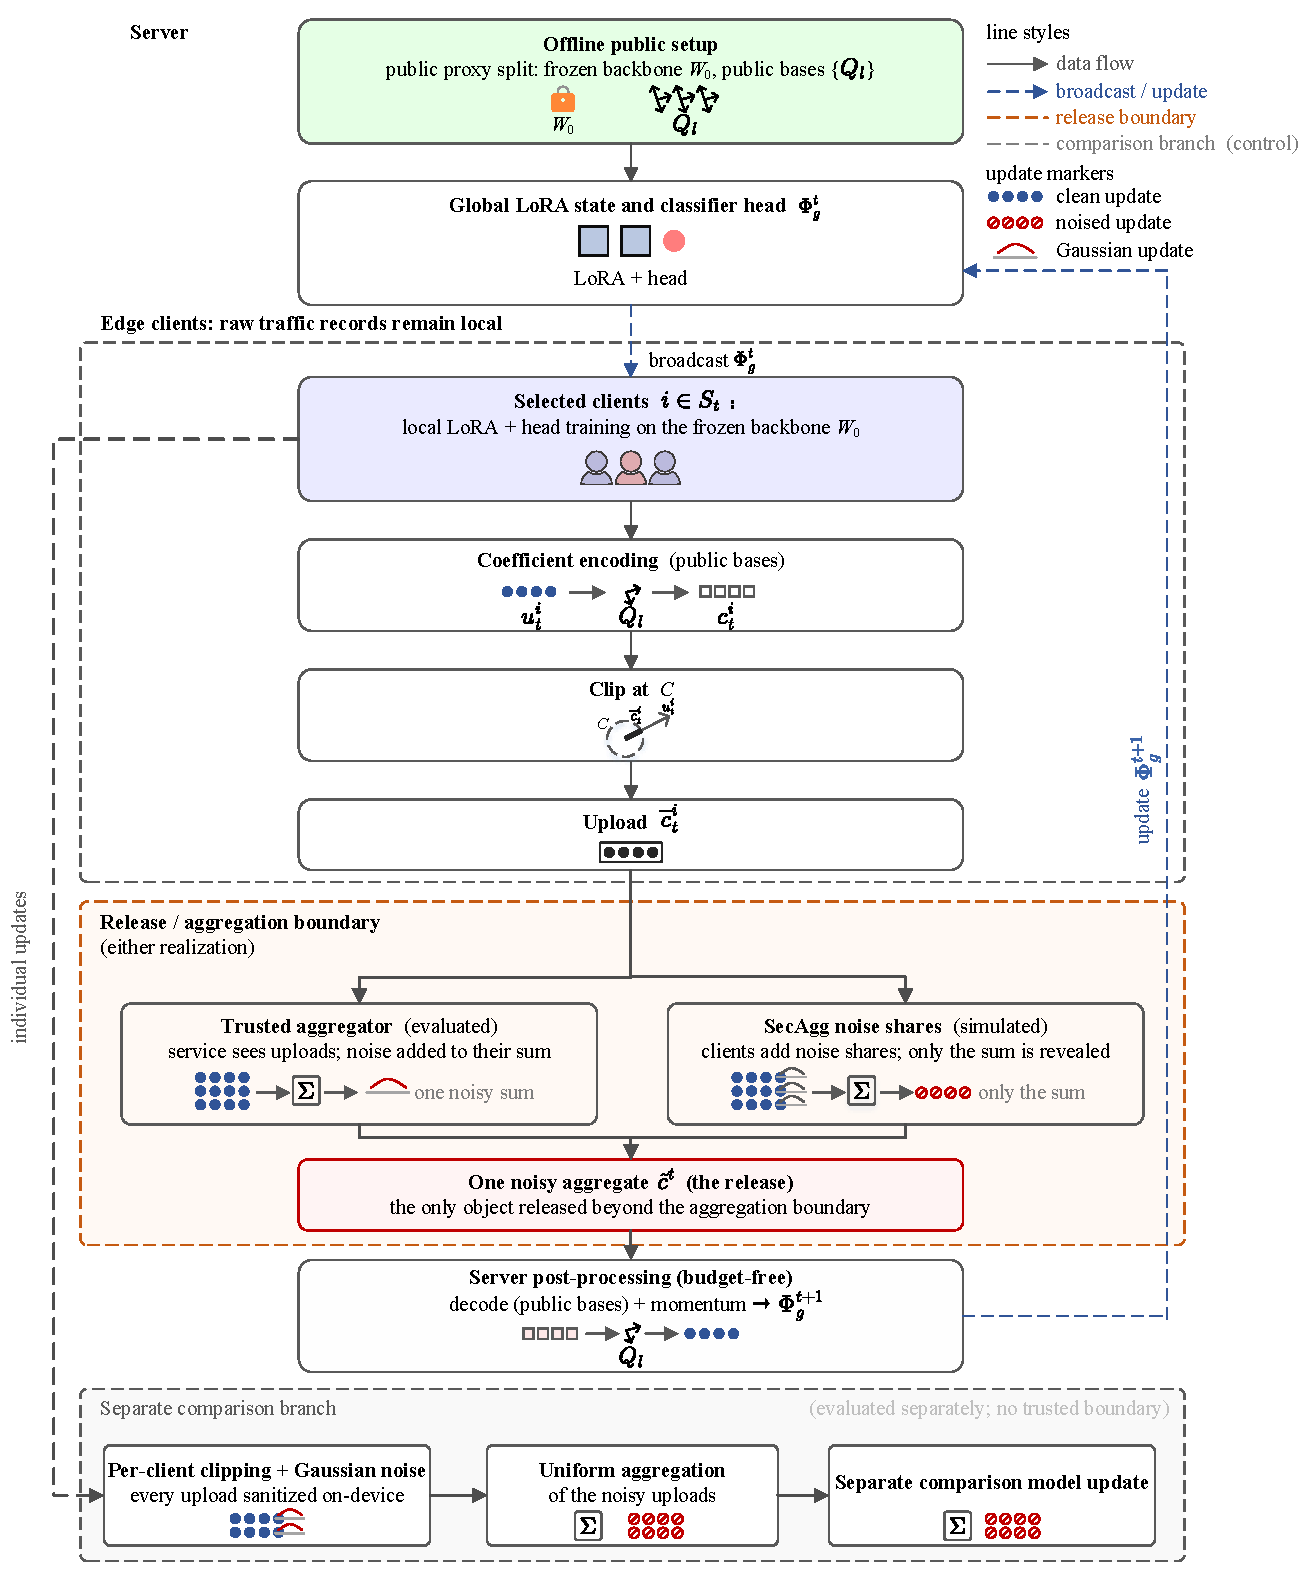
\includegraphics[width=\linewidth]{jiagoutu.pdf}
\caption{The \MethodinCaption\ release protocol (\cref{subsec:agg-release} -- \cref{subsec:perclient}). Both realizations release the same noisy aggregate $\tilde c^t$, the only data-dependent object released per round; raw traffic records remain local throughout. The gray strip at the bottom summarizes the separate per-client comparison branch, evaluated outside the release boundary as the no-trust alternative. The public bases fix the representation space of the aggregate branch; protocol-matched comparisons attribute no utility advantage to their provenance over same-dimension random bases (\cref{sub:attribution}).}
\label{fig:framework} % 给图编号，方便引用
\end{figure*}
\par
\begin{algorithm}[tbp]
\caption{\method\ round procedure (Overview)}
\label{alg:overview}
\begin{algorithmic}[1]
\Require frozen backbone $W_0$; public bases $\{Q_\ell\}$ (Basis); client datasets $\{D_i\}$; public selection rule; total $(\epsilon,\delta)$; rounds $T$; clip $C$; momentum $\beta$; cap $n_{\max}$; branch configuration (\cref{tab:branchconfigs}); mode $\in$ \{aggregate, per-client\}
\State Initialize the zCDP ledger $\mathcal{Z}$ with budget $\rho$; momentum $v^0$; global state $\Phi_g^0$
\For{round $t=1,\ldots,T$}
\State Broadcast $\Phi_g^{t-1}$ to the selected set $\mathcal{S}_t$ \Comment{public sampling}
\For{each client $i\in\mathcal{S}_t$ in parallel}
\State Fine-tune locally on $D_i$; form the adapter update $u_i^t$
\If{mode $=$ per-client}
\State Clip and Gaussian-sanitize $u_i^t$; upload \Comment{the server sees only noised uploads}
\Else
\State Encode $c_i^t\gets\mathrm{vec}(\{Q_\ell^\top u_{i,\ell}^t\}_\ell)$; clip to norm $C$; upload $\bar c_i^t$
\EndIf
\EndFor
\If{mode $=$ aggregate}
\State \textbf{Aggregate} (\cref{alg:aggrelease}) releases the noised uniform-weight sum
\Else
\State The server sums the sanitized uploads with uniform weights
\EndIf
\State Decode; momentum update; $\Phi_g^t\gets\Phi_g^{t-1}+v^t$ \Comment{post-processing, budget-free}
\State Append the branch debit to $\mathcal{Z}$; exclude clients at budget or cap
\EndFor
\State \Return $\Phi_g^{T}$, ledger $\mathcal{Z}$
\end{algorithmic}
\end{algorithm}
\par
\subsection{Public Subspace Representation and Client-Side Preprocessing}
\label{subsec:publicsubspace}
\par
Before federated training, a fixed orthonormal basis $Q_\ell\in\mathbb{R}^{d_\ell\times k_\ell}$ is constructed for every transmitted tensor $\ell$ by Basis (\cref{alg:subspace}) from a singular value decomposition (SVD) of update statistics on a disjoint public split; the construction is deterministic given the split and the completion seed, and the basis is shipped with the artifact.
\par
This split is also used for backbone pre-training and the FLTrust root update. The basis is fixed before training, and the plain FedLoRA reference trains on the same public checkpoint, so the projection
\begin{equation}
c_i^t=\mathrm{vec}\big(\{Q_\ell^\top u_{i,\ell}^t\}_\ell\big)\in\mathbb{R}^{K}
\end{equation}
is a public, data-independent linear map that consumes no privacy budget. Client updates are clipped in coefficient space, $\bar c_i^t=c_i^t\cdot\min\{1,C/\|c_i^t\|_2\}$, which matches the clipping norm to the coefficient-norm distribution rather than the ambient one and bounds the sensitivity of the aggregate release.
\par
\begin{algorithm}[tbp]
\caption{Public-basis construction (Basis, offline)}
\label{alg:subspace}
\begin{algorithmic}[1]
\Require stratified public split $\mathcal{D}_{\mathrm{pub}}$; pretrained
checkpoint; per-tensor dimension $k_\ell$; completion seed
\State Partition $\mathcal{D}_{\mathrm{pub}}$ into $S$ disjoint shards
\For{each shard}
\State One fine-tuning pass from the public checkpoint gives an update $u^{(s)}$
\EndFor
\For{each transmitted tensor $\ell$}
\State SVD of the stacked shard updates; keep the leading $k_\ell$ singular vectors
\State Seeded orthogonal completion to $Q_\ell\in\mathbb{R}^{d_\ell\times k_\ell}$
\EndFor
\State \Return $\{Q_\ell\}$, fixed for all clients and rounds
\end{algorithmic}
\end{algorithm}
\par
\subsection{Aggregate-Release Branch}
\label{subsec:agg-release}
\par
In the aggregate branch, the selected clients transmit clipped coefficient vectors to the aggregation boundary. The aggregation weights are fixed a priori as $w_i^t=1/|\mathcal{S}_t|$ for every selected client $i$ in round $t$, where $\mathcal{S}_t$ is the selected set. Uniform weights make the sensitivity analysis exact and keep the aggregation rule a plain sum, realizable without exposing per-client values. The server adds one Gaussian perturbation to the uniform-weight sum per round:
\begin{equation}
\tilde c^t=\sum_i w_i^t\bar c_i^t+\eta^t,\qquad \eta^t\sim\mathcal{N}(0,\sigma_t^2 I_K).
\end{equation}
The per-release noise $\sigma_t$ is calibrated by the zero-concentrated DP (zCDP) accountant of \cref{sec:analysis}, which avoids the $\epsilon\le 1$ restriction of the classical Gaussian bound; the sensitivity derivation and the composition analysis are stated there.
\par
Aggregate implements the release in the two realizations of \cref{subsec:adversary}. A client that drops out after adding its share does not affect the guarantee, and the consistency argument is given in the supplementary material.
\par
\begin{algorithm}[tbp]
\caption{Aggregate release (Aggregate)}
\label{alg:aggrelease}
\begin{algorithmic}[1]
\Require clipped coefficients $\{\bar c_i^t\}_{i\in\mathcal{S}_t}$; ledger
$\mathcal{Z}$
\State Uniform weights $w_i^t\gets 1/|\mathcal{S}_t|$; sensitivity
$\Delta^t\gets 2C/|\mathcal{S}_t|$
\State $\sigma_t\gets\Delta^t/\sqrt{2\rho_r}$ with $\rho_r=\rho/T$
\State \emph{Trusted mode:} the service sums the uploads and adds
$\mathcal{N}(0,\sigma_t^2I_K)$
\Comment{uploads visible to the service}
\State \emph{SecAgg mode (simulated):} each client uploads $w_i^t\bar c_i^t$
plus an independent noise share of variance $\sigma_t^2/|\mathcal{S}_t|$
\Comment{shares sum to $\mathcal{N}(0,\sigma_t^2I_K)$; no plaintext sum
server-side}
\State \Return the released sum $\tilde c^t$
\end{algorithmic}
\end{algorithm}
\par
\paragraph{Decoding and server update}
The server decodes the sanitized coefficients back to adapter-update tensors, tensor by tensor, as $\widehat{\Delta\theta}_\ell=Q_\ell\tilde c^t_\ell$; the decoded update $\widetilde u^t=\mathrm{vec}(\{\widehat{\Delta\theta}_\ell\}_\ell)$ lives in the adapter-update space. The server then maintains an exponential moving average of the released, decoded updates,
\begin{equation}
v^t=\beta\, v^{t-1}+(1-\beta)\,\widetilde u^t,\qquad
\Phi_g^{t}=\Phi_g^{t-1}+v^t,
\end{equation}
with $\beta$ as a deployment hyperparameter and $v^1=\widetilde u^1$, with the recursion applied from $t=2$. Because the recursion is a deterministic function of already released aggregates, it is budget-free post-processing in the sense of \cref{prop:composition}. It low-pass filters the per-round Gaussian perturbations while preserving the coherent optimization direction. The momentum coefficient is a deployment hyperparameter selected on the validation split, subject to a protocol-length constraint ($\beta\lesssim 1-1/T$); its empirical effect is quantified in \cref{sub:attribution}.
\par
\subsection{Per-Client Comparison Branch}
\label{subsec:perclient}
\par
The per-client release is the no-trust comparison branch of the protocol. It shares the ledger discipline and the local training procedure of the main configuration, but each client clips and Gaussian-sanitizes its own update before upload. Let $u_i^t$ be the client's effective adapter update: the implied weight updates $\Delta W_\ell$ together with the classifier-head parameters. The released update is clipped,
\begin{equation}
\bar u_i^t=u_i^t\min\left(1,\frac{C}{\|u_i^t\|_2+10^{-12}}\right),
\end{equation}
with a fixed clipping norm $C$, and sanitized,
\begin{equation}
\widetilde u_i^t=\bar u_i^t+\mathcal{N}(0,\sigma_{i,t}^2 I),\qquad
\widetilde u^t=\sum_i w_i^t\widetilde u_i^t,
\end{equation}
where each client-side Gaussian scale $\sigma_{i,t}$ is calibrated from the configured total $(\epsilon,\delta)$ budget and the per-client upload cap, and the implementation records the resulting privacy ledger and round-level noise statistics.
\par
The representation space is part of the configuration under comparison rather than a fixed choice; the evaluated variants are tabulated in \cref{tab:branchconfigs}. The sanitized update is factorized back into the LoRA form for transmission, so the wire object remains a rank-preserving LoRA representation and server-side aggregation needs no projection decode; the per-client release procedure is reproduced in the supplementary material.
\par
The principal privacy claim of this branch applies to each sanitized per-client release and to its subsequent aggregation as post-processing. It does not protect an individual clean delta that is sent to a curious server; the formal guarantee and ledger details are stated in \cref{sec:analysis}. Optional extensions attach to this branch and to a trusted aggregator (supplementary material); none enters the formally analyzed aggregate release.
\par
\section{Privacy and Complexity Analysis}
\label{sec:analysis}
\par
For readers outside differential privacy, the analysis uses the following vocabulary. Client-level DP under replacement adjacency asks the release to be statistically indistinguishable when one client's entire contribution is replaced; $\epsilon$ bounds the multiplicative change in outcome probabilities and $\delta$ the residual failure probability. Clipping each update to norm $C$ caps the induced shift at twice the clip, $2C$ ($2C/|\mathcal{S}_t|$ for the uniform-weight aggregate), the sensitivity against which Gaussian noise is calibrated. Basic composition adds the per-release $\epsilon$ across rounds and exhausts a fixed budget quickly; zCDP tracks a per-release parameter $\rho$ that converts to a tighter total $(\epsilon,\delta)$, and the choice between the two composition rules is itself part of the studied design space.
\par
Both branches are analyzed under the assumptions fixed in \cref{subsec:adversary}: client-level DP under replacement adjacency as the privacy objective, the visibility and trust boundaries of \cref{tab:trust}, the data-independent public bases of \cref{subsec:publicsubspace}, and public sampling with uniform weights and accounting that covers arbitrary repeated participation. One assumption is added here: the Gaussian noise derives from an unpredictable, deployment-grade random source not disclosed to the adversary. The only data-dependent object released in round $t$ is the sanitized release of the active branch.
\par
\subsection{Per-client release}
\par
A randomized mechanism $\mathcal{M}$ satisfies $(\epsilon,\delta)$ client-level differential privacy for a released upload if adjacent federated datasets $D$ and $D'$ differ in the complete local dataset of one client, with all other clients unchanged, and for any output set $S$,
\begin{equation}
\Pr[\mathcal{M}(D)\in S]\leq e^\epsilon \Pr[\mathcal{M}(D')\in S]+\delta .
\end{equation}
If an update mapping has $\ell_2$ sensitivity $S$, the Gaussian mechanism releases $g(D)+\mathcal{N}(0,\sigma^2I)$ with
\begin{equation}
\sigma \geq \frac{S\sqrt{2\log(1.25/\delta)}}{\epsilon},
\end{equation}
the classical sufficient condition, stated for $0<\epsilon<1$; the exact Gaussian mechanism extends the construction to all $\epsilon>0$.
\par
\begin{proposition}[Per-client release and sequential composition (standard)]
\label{thm:perround}
Let $C$ be the client update clipping norm and let $\bar u_i^t$ be the
clipped update of client $i$. Under replacement adjacency, the sensitivity
of this update is at most $2C$. If the client releases
\begin{equation}
\begin{aligned}
&\widetilde u_i^t = \bar u_i^t + \mathcal{N}(0,\sigma_{i,t}^2 I) \\
&\qquad\text{ with }
\sigma_{i,t} \geq \frac{2C\sqrt{2\log(1.25/\delta_{i,t})}}{\epsilon_{i,t}},
0<\epsilon_{i,t}<1,
\end{aligned}
\end{equation}
then each sanitized upload satisfies $(\epsilon_{i,t},\delta_{i,t})$
client-level DP, and the sequence of a client's uploads satisfies
$(\sum_t \epsilon_{i,t}, \sum_t \delta_{i,t})$ client-level DP. Any weighted
aggregation, rank projection, factorization, or evaluation performed only on
sanitized updates is post-processing.
\end{proposition}
\par
\begin{proof}
See the supplementary material for the full proof.
\end{proof}
\par
\paragraph{Participation protocol and budget ledger}
The per-client guarantee is stated per released upload and must be paired
with a protocol that caps how often a client releases. The evaluated protocol
enforces three rules. First, client sampling in each round is determined by
the public selection rule and the transcript only, never by private data
values, so a client's participation pattern is independent of its dataset.
Second, each client is allowed at most $n_{\max}$ uploads over the
protocol; the per-round selection size and the protocol length are fixed in
advance, so no client can be selected beyond its cap. Third, the aggregation service maintains
a per-client ledger of released debits. In the evaluated per-client
configuration, each upload debits a per-upload zCDP cost calibrated at the
replacement sensitivity $2C$ from the recorded noise. A client's at most
$n_{\max}$ uploads therefore compose in zCDP below the total budget, and the
converted $(\epsilon,\delta)$ stays within the reported total
(\cref{tab:branchconfigs}). The naive baseline instead calibrates each
upload at a nominal per-upload budget under basic composition, with the
noise fixed by the classical Gaussian formula
(\cref{tab:branchconfigs}). The classical sufficient condition behind
that formula requires $\epsilon_r<1$, so the nominal per-upload budget is
not itself a formal guarantee. The exact zCDP accounting of the recorded
noise at the same sensitivity composes below the reported total, which is
the guarantee we claim for this baseline.
A client
whose next upload would exceed its composed budget, or whose upload count
would reach the cap, is excluded from further selection for the
remainder of the protocol. The guarantee of \cref{thm:perround}
therefore always composes to at most the reported $(\epsilon,\delta)$, and
the ledger check is a function of already-recorded release parameters, not of
private data. If deployments deviate from these rules, for example by
admitting clients more than $n_{\max}$ times under a different sampling
schedule, the total budget must be re-derived from the realized ledger rather
than taken from this paper.
\par
\paragraph{Conventions}
All \method\ per-client calibrations use the replacement sensitivity $2C$ of
\cref{thm:perround}; under the enforced upload cap, the composed
zCDP ledger evaluates below the reported total $(\epsilon,\delta)$
(\cref{tab:branchconfigs}), which
therefore remains a valid upper bound. The naive baseline composes per-upload
nominal basic budgets and is reported at its composed value
(\cref{tab:branchconfigs}). All per-client guarantees are stated
in the effective adapter-update space: the flattened concatenation of the
implied weight updates $\Delta W_\ell=B_\ell A_\ell$ and the
classifier-head parameters ($83{,}970$ entries,
\cref{tab:ktensors}); clipping and Gaussian noise act
in this space, or, whenever a public basis is used, in its coefficient-space
image. Any update decoded from a sanitized release, in whatever
representation, and the adapted model itself are post-processing
(\cref{thm:perround,prop:composition}); no guarantee
is claimed for objects computed from plaintext updates outside the release
boundary. The aggregate branch of \cref{subsec:agg-theory} instead
moves the release boundary to the aggregate, so the per-client guarantee is
not claimed for it.
\par
\subsection{Aggregate release}
\label{subsec:agg-theory}
\par
The main configuration of \method\ releases the aggregate of
\cref{subsec:agg-release}.
\par
The noise scale of the aggregate release is calibrated by the zCDP
accountant. With total budget $(\epsilon,\delta)$, define the total zCDP
budget
\begin{equation}
\rho=\Big(\sqrt{\ln(1/\delta)+\epsilon}-\sqrt{\ln(1/\delta)}\Big)^2,
\qquad
\rho_r=\frac{\rho}{T},
\label{eq:zcdp-rho}
\end{equation}
and set the per-round noise scale
\begin{equation}
\sigma_t=\frac{\Delta^t}{\sqrt{2\rho_r}}=\frac{2C}{|\mathcal{S}_t|\sqrt{2\rho/T}},
\label{eq:zcdp-sigma}
\end{equation}
where $\Delta^t=2C/|\mathcal{S}_t|$ is the replacement sensitivity of the
weighted sum. The budget allocation and ledger update that instantiate
\cref{thm:perround,prop:round,prop:composition} in both release
branches are reproduced as Algorithms~S1 and~S2 in the supplementary
material: the aggregate split of the total zCDP budget across
rounds, and the per-client per-upload debits. The two branches allocate differently by
design: the aggregate branch splits the total zCDP budget evenly over the
$T$ planned rounds, whereas the per-client branch debits each upload a
per-upload zCDP cost calibrated at the same replacement sensitivity and caps
a client at $n_{\max}$ uploads, so the composed per-client cost stays below
the total budget. The naive baseline of \cref{tab:branchconfigs} instead
composes per-upload basic budgets and is reported at its composed value.
\par
\begin{proposition}[Per-round aggregate release, conditioned on the transcript]
\label{prop:round}
Under the release model, fix any round $t$ and condition on an arbitrary
realized transcript prefix $h_{t-1}=(\tilde c^1,\dots,\tilde c^{t-1})$ of
earlier releases. Given $h_{t-1}$, the round-$t$ mechanism
\begin{equation}
\begin{aligned}
& \mathcal{M}_t(D\mid h_{t-1})
= \sum_{i\in\mathcal{S}_t(h_{t-1})}
\frac{\bar c_i^t(D,h_{t-1})}{|\mathcal{S}_t(h_{t-1})|}
+ \eta^t,\\
&\qquad\eta^t \sim \mathcal{N}\!\left(0,\sigma_t^2 I_K\right),
\quad
\sigma_t = \frac{\Delta^t}{\sqrt{2\rho_r}},
\end{aligned}
\end{equation}
with $\Delta^t=2C/|\mathcal{S}_t(h_{t-1})|$ and $\rho_r=\rho/T$ from
\eqref{eq:zcdp-rho}, satisfies $\rho_r$-zCDP conditionally on $h_{t-1}$.
\end{proposition}
\par
\begin{proof}
See the supplementary material for the full proof.
\end{proof}
\par
\begin{proposition}[Composition, budget conversion, and post-processing]
\label{prop:composition}
Under the release model, the $T$-round transcript
$(\mathcal{M}_1,\dots,\mathcal{M}_T)$ is jointly $\rho$-zCDP with
$\rho = T\rho_r$, and with $\rho$ chosen as in \eqref{eq:zcdp-rho} the
released aggregates satisfy the reported $(\epsilon,\delta)$-DP bound. Any function computed solely from the
released aggregates $\{\tilde c^s\}_{s \le t}$, including the decoded adapter
update, the server momentum state $v^t$, the updated global state
$\Phi_g^t$, the evaluation metrics, and, in the per-client release, the
history-based privacy controller and anomaly thresholds, preserves this
guarantee and consumes no additional privacy budget.
\end{proposition}
\par
\begin{proof}
See the supplementary material for the full proof.
\end{proof}
\par
\paragraph{Anomaly-aware extension}
\cref{prop:round,prop:composition} rely on the
data-independent weights of the release model. For the trusted-aggregator
extension that replaces them with anomaly-aware weights, an unconditional
worst-case bound of $\Delta = 2C$ holds for any simplex weights, because a
convex combination of norm-$C$ vectors has norm at most $C$ and the
replacement diameter is therefore $2C$. Calibrating to this bound scales the
noise by roughly $|\mathcal{S}_t|$, and weights computed only from public
data or previously released aggregates are post-processing and retain
$2Cw_{\max}$. The extension consequently falls outside the formal results
and carries the no-DP-claim boundary stated in
\cref{subsec:agg-release}.
\par
Under the release model, the released aggregate satisfies the reported
$(\epsilon,\delta)$-DP bound. The two release systems protect different
objects, namely each sanitized upload versus the sanitized aggregate
(\cref{subsec:adversary}); their guarantees must not be conflated. The
influence-suppression property of the trusted-aggregator anomaly-weight
extension is proven in the supplementary material; the main configuration
does not use anomaly weights.
\par
\subsection{Cost Analysis}
\label{subsec:cost}
\par
\paragraph{Utility of rank-preserving projection}
The rank-preserving projection also bounds the utility loss of the protected
path. Let $\bar{\Delta W}_i^\ell$ be the clipped
clean adapter update and let $\Delta W_{i,\mathrm{priv}}^\ell =
\bar{\Delta W}_i^\ell + E_i^\ell$ be the noisy update before projection.
Because $\mathcal{P}_r(\cdot)$ is the best rank-$r$ approximation in
Frobenius norm,
\begin{equation}
\|\widehat{\Delta W}_i^\ell-\bar{\Delta W}_i^\ell\|_F
\leq
2\|E_i^\ell\|_F+
\|\bar{\Delta W}_i^\ell-\mathcal{P}_r(\bar{\Delta W}_i^\ell)\|_F .
\end{equation}
When the clean LoRA update is already close to rank $r$, the projection
error is therefore controlled mainly by the calibrated privacy noise, and
the mechanism protects the effective adapter update while keeping the
transmitted object in the low-rank LoRA form.
\par
\paragraph{Communication}
If a layer has dimensions $d_{\mathrm{out}}\times d_{\mathrm{in}}$ and rank
$r$, the uploaded protected adapter factors contain
$r(d_{\mathrm{out}}+d_{\mathrm{in}})$ parameters rather than
$d_{\mathrm{out}}d_{\mathrm{in}}$ parameters, so \method\ preserves the
parameter-efficiency advantage of LoRA even though perturbation is
calibrated in the effective adapter-update space. Let $M=|\mathcal{S}_t|$ be
the number of selected clients in a round, $K$ the released coefficient
dimension, and $P_r$ the transmitted LoRA-plus-head parameter count. With
each coefficient transmitted as a raw 32-bit value, every participating
client sends $4K$ bytes per round, the total upstream coefficient payload is
$4KM$ bytes, and the aggregation boundary releases one $4K$-byte aggregate.
These counts exclude downlink state, protocol headers, cryptographic
framing, key exchange, metadata, and dropout recovery, so they concern the
raw model payload only. A Bonawitz-style secure-aggregation layer would, by
analytical estimate, roughly triple the per-client coefficient payload;
this estimate is analytical, not an implementation result.
\par
\paragraph{Complexity}
Client clipping and Gaussian sanitization are $O(P_r)$, rank projection is a
truncated SVD on matrix-shaped LoRA components, and weighted aggregation is
$O(KP_r)$; head tensors bypass matrix projection. Anomaly descriptors and
data-dependent weighting belong only to the per-client release or the
trusted-aggregator extension. The fixed-weight configuration adds
client-side encoding and coefficient clipping, one aggregate perturbation,
decoding, and momentum post-processing.
\par
\section{Experimental Evaluation}
\label{sec:evaluation}
\par
This section answers the question posed in the Introduction. \cref{sub:setup} fixes the experimental environment, datasets, model, baselines, metrics, hyperparameters, and statistical protocol. \cref{sub:operating} reports the main utility and privacy results, asking whether each release design retains usable detection quality. \cref{sub:attribution} attributes the observed privacy--utility gap to the release boundary, the release dimension, the accounting and clipping configuration, the server momentum, and the basis provenance. \cref{sub:boundaries,sub:scalability} map the boundaries of these conclusions across the privacy budget, client heterogeneity, adapter rank, and communication and computational cost. \cref{sub:robustness} reports the malicious-client stress tests. Repeated runs are reported as mean and sample standard deviation.
\par
\subsection{Experimental Setup}
\label{sub:setup}
\par
\cref{tab:setup} fixes the setup shared by all experiments; this
subsection states the comparison principles and the data limitations.
\par
\par
\begin{table*}[pos=tbp]
\centering
\rmfamily
\small
\caption{Configuration of every protected branch; PC-DP abbreviates per-client DP.}
\label{tab:branchconfigs}
\begin{tblr}
{
columns={co=-1},
cells={valign=m,halign=c},
columns={colsep=4pt},
rows={rowsep=2pt},
rows={ht=0pt},
stretch=0,
hline{1,Z}={wd=.08em},
hline{2}={wd=.05em},
cells={font=\fontsize{9pt}{8pt}},
row{1}={font=\bfseries\boldmath\fontsize{9pt}{8pt}},
row{even[2]}={bg=gray9!35},
}
Configuration & {Protected\\object} & Release space & Noise calibration \\
FedLoRA & {none\\(reference)} & full adapter update & none \\
{DP-FedLoRA\\(naive)} & {each\\upload} & {full ambient update,\\no basis ($83{,}970$)} & $C=1.0$; $\sigma=5.123$; nominal basic composition, per-upload $(\epsilon_r,\delta_r)\allowbreak=(2,2.5{\times}10^{-6})$; composed $(8,10^{-5})$, exact zCDP $\epsilon{\approx}4.05$; cap $n_{\max}=4$ \\
{PC-DP\\(tight)} & {each\\upload} & {public-basis\\coefficients, $K=6{,}970$} & $C=0.05$; $\sigma=0.1544$; zCDP, $\epsilon{\approx}7.1\le8$; cap $n_{\max}=4$ \\
{\method\\(main, $K=146$)} & {one aggregate\\per round} & {layerwise basis,\\$k_\ell=48$ (146)} & $\sigma=0.0309$; $2C/|\mathcal{S}_t|=0.01$; zCDP over $T=20$ \\
{\method\ (sweep\\anchor, $K=98$)} & {one aggregate\\per round} & {global basis,\\$k_\ell=32$ (98)} & $\sigma=0.0309$; sweep anchor; $\beta=0.98$ \\
\end{tblr}
\end{table*}
\par
\par
\begin{table}[pos=tbp]
\centering
\rmfamily
\small
\caption{Experimental setup shared by all experiments; per-branch
protection and noise calibration are fixed in
\cref{tab:branchconfigs}, and the basis allocation in
\cref{tab:ktensors}.}
\label{tab:setup}
\begin{tblr}
{
columns={co=-1},
cells={valign=m,halign=c},
cell{2-Z}{Z}={valign=m,halign=j},
columns={colsep=3pt},
rows={rowsep=2pt},
rows={ht=0pt},
stretch=0,
hline{1,Z}={wd=.08em},
hline{2}={wd=.05em},
cells={font=\fontsize{9pt}{8pt}},
row{1}={font=\bfseries\boldmath\fontsize{9pt}{8pt}},
row{even[2]}={bg=gray9!35},
}
Category & Setting\\
Environment & PyTorch on CPU; fixed package versions, resolved configurations, and seeds make every run replayable\\
Optimization & SGD; learning rate $10^{-3}$, weight decay $10^{-4}$, batch 128, one local epoch per round\\
Datasets & UNSW-NB15 \cite{moustafa2015unsw}: 257{,}673 records, 199 features, official 175{,}341/82{,}332 split; CICIDS2017 \cite{sharafaldin2018cicids}: 2{,}830{,}743, 77, stratified 2{,}264{,}595/566{,}148; Edge-IIoT \cite{ferrag2022edgeiiot}: 157{,}800, 55, stratified 126{,}240/31{,}560; all binary benign-versus-attack\\
Model & two-layer tabular MLP, hidden 256/128; 6{,}970 trainable parameters; rank-8 LoRA factors plus a 258-parameter head\\
Federation & 50 logical clients, Dirichlet $\alpha=0.5$; 10 clients sampled per round; $T=20$ rounds; public fraction $0.1$\\
Privacy & composed $(\epsilon,\delta)=(8,10^{-5})$; $\epsilon\in\{2,4,8,16\}$ in the budget sweep; coefficient-space clipping $C=0.05$ (aggregate, tightened per-client), update-space $C=1.0$ (naive, remaining baselines)\\
Seeds & main contrasts $\{7,17,27,37,47\}$ ($n=5$); sensitivity families $\{7,17,27\}$ ($n=3$)\\
Baselines & FedLoRA, Clipped, DP-FedLoRA, Median, Trimmed Mean, Krum, FLTrust; head-only and full fine-tuning (Edge-IIoT)\\
\end{tblr}
\end{table}
\par
\par
\paragraph{Environment}
All experiments run in PyTorch on CPU; the simulator fixes package versions, resolved configurations, and seeds, so utility measurements and Gaussian samples are replayable. Formal deployment requires an unpredictable noise source.
\par
\paragraph{Datasets}
The evaluation uses the binary intrusion-detection tasks of UNSW-NB15, CICIDS2017, and Edge-IIoT; record counts, feature dimensions, and splits are listed in \cref{tab:setup}.
\par
\paragraph{Preprocessing}
Identifier-like columns are dropped, non-finite entries are zero-filled, categorical columns are one-hot encoded with a missing indicator, and all features are standardized with a scaler fitted on the public pre-training fraction only, so no test statistics enter training.
\par
\paragraph{Split integrity} The official UNSW-NB15 split is kept as released. For CICIDS2017 the split is stratified random at record level; because the underlying flows are exported in five-tuple windows, a flow-disjoint or time-ordered split is \emph{not} guaranteed. In the standard split, $13.4\%$ of test records share an exact feature-vector duplicate with the training side ($28.6\%$ among attack records). \cref{app:fdrep} quantifies this overlap and shows that the attribution contrasts are preserved under a duplicate-group-disjoint replication, while absolute levels move with test-set composition.
\par
\paragraph{Model and federation} The private training data are partitioned among 50 logical clients with Dirichlet label skew~\cite{hsu2019measuring}; a client is a logical traffic domain rather than a validated one-to-one gateway, and the partition is a controlled non-IID stress test rather than a reproduction of natural network heterogeneity. The backbone is frozen, and only the LoRA factors and the classifier head are trained locally. Model, federation, optimization, and seed settings are listed in \cref{tab:setup}, and any single-seed run is explicitly labelled; \cref{tab:ktensors} lists the per-tensor ambient dimensions of the transmitted tensors and the public-basis allocation for the two coefficient budgets; for the experiments, the public split is partitioned into $S=64$ shards (Basis, \cref{alg:subspace}).
\par
\begin{table}[pos=tbp]
\centering
\rmfamily
\small
\caption{Per-tensor ambient dimensions $d_\ell$ of the transmitted tensors and the public-basis allocation of the $K=98$ sweep anchor; the main layerwise configuration uses $k_\ell=48$ per weight tensor ($K=146$).}
\label{tab:ktensors}
\begin{tblr}
{
columns={co=-1},
cells={valign=m,halign=c},
columns={colsep=3pt},
rows={rowsep=2pt},
rows={ht=0pt},
stretch=0,
hline{1,Z}={wd=.08em},
hline{2}={wd=.05em},
cells={font=\fontsize{9pt}{8pt}},
row{1}={font=\bfseries\boldmath\fontsize{9pt}{8pt}},
row{even[2]}={bg=gray9!35},
}
Transmitted tensor $\ell$ & $d_\ell$ & $k_\ell$ (sweep) & $k_\ell$ (main)\\
First-layer weight update & 50{,}944 & 32 & 48\\
Second-layer weight update & 32{,}768 & 32 & 48\\
Classifier head weight & 256 & 32 & 48\\
Classifier head bias & 2 & 2 & 2\\
Total ambient entries & 83{,}970 & & \\
Total released coefficients $K$ & --- & 98 & 146\\
\end{tblr}
\end{table}
\par
\par
\begin{table*}[pos=tbp]
\centering
\rmfamily
\small
\caption{Main clean-task results: mean $\pm$ sample standard deviation, five
seeds; the Edge-IIoT block is a three-seed replication. Best Macro-F1 per
block in bold.}
\label{tab:mainresults}
\begin{tblr}
{
columns={co=-1},
cells={valign=m,halign=c},
columns={colsep=6pt},
rows={rowsep=2pt},
rows={ht=0pt},
stretch=0,
hline{1,Z}={wd=.08em},
hline{2,11,20}={wd=.05em},
cells={font=\fontsize{9pt}{8pt}},
row{1}={font=\bfseries\boldmath\fontsize{9pt}{8pt}},
cell{8,19,26}{3-5}={font=\bfseries\boldmath\fontsize{9pt}{8pt}},
cell{10,19,26}{2}={font=\bfseries\boldmath\fontsize{9pt}{8pt}},
row{even[2]}={bg=gray9!35},
}
Dataset & Method & Accuracy & Macro-F1 & FAR & MIA AUC\\
CICIDS2017 & FedLoRA & 0.9784 $\pm$ 0.0078 & 0.9649 $\pm$ 0.0137 & 0.0061 $\pm$ 0.0053 & 0.4979 $\pm$ 0.0005\\
CICIDS2017 & Clipped & 0.9794 $\pm$ 0.0040 & 0.9668 $\pm$ 0.0066 & 0.0075 $\pm$ 0.0027 & 0.4974 $\pm$ 0.0011\\
CICIDS2017 & DP-FedLoRA & 0.4050 $\pm$ 0.2130 & 0.3608 $\pm$ 0.1658 & 0.6548 $\pm$ 0.3155 & 0.4987 $\pm$ 0.0064\\
CICIDS2017 & Median & 0.9823 $\pm$ 0.0040 & 0.9722 $\pm$ 0.0063 & 0.0140 $\pm$ 0.0073 & 0.4969 $\pm$ 0.0011\\
CICIDS2017 & Trimmed Mean & 0.9823 $\pm$ 0.0044 & 0.9722 $\pm$ 0.0069 & 0.0139 $\pm$ 0.0070 & 0.4967 $\pm$ 0.0010\\
CICIDS2017 & Krum & 0.9754 $\pm$ 0.0085 & 0.9620 $\pm$ 0.0116 & 0.0209 $\pm$ 0.0178 & 0.4973 $\pm$ 0.0008\\
CICIDS2017 & FLTrust & 0.9831 $\pm$ 0.0042 & 0.9733 $\pm$ 0.0069 & 0.0124 $\pm$ 0.0019 & 0.4968 $\pm$ 0.0013\\
CICIDS2017 & PC-DP (tight accounting) & 0.9524 $\pm$ 0.0119 & 0.9202 $\pm$ 0.0228 & 0.0142 $\pm$ 0.0038 & 0.4998 $\pm$ 0.0014\\
CICIDS2017 & \method\ (ours) & 0.9758 $\pm$ 0.0022 & 0.9618 $\pm$ 0.0033 & 0.0158 $\pm$ 0.0038 & 0.4982 $\pm$ 0.0011\\
UNSW-NB15 & FedLoRA & 0.8207 $\pm$ 0.0103 & 0.8063 $\pm$ 0.0134 & 0.3883 $\pm$ 0.0340 & 0.5801 $\pm$ 0.0031\\
UNSW-NB15 & Clipped & 0.8225 $\pm$ 0.0114 & 0.8085 $\pm$ 0.0146 & 0.3835 $\pm$ 0.0371 & 0.5798 $\pm$ 0.0035\\
UNSW-NB15 & DP-FedLoRA & 0.5483 $\pm$ 0.0728 & 0.4533 $\pm$ 0.1387 & 0.4583 $\pm$ 0.4795 & 0.5053 $\pm$ 0.0508\\
UNSW-NB15 & Median & 0.8251 $\pm$ 0.0074 & 0.8118 $\pm$ 0.0094 & 0.3770 $\pm$ 0.0241 & 0.5833 $\pm$ 0.0012\\
UNSW-NB15 & Trimmed Mean & 0.8262 $\pm$ 0.0079 & 0.8132 $\pm$ 0.0101 & 0.3736 $\pm$ 0.0258 & 0.5847 $\pm$ 0.0017\\
UNSW-NB15 & Krum & 0.8290 $\pm$ 0.0166 & 0.8166 $\pm$ 0.0206 & 0.3620 $\pm$ 0.0557 & 0.5842 $\pm$ 0.0017\\
UNSW-NB15 & FLTrust & 0.8157 $\pm$ 0.0027 & 0.8000 $\pm$ 0.0036 & 0.4043 $\pm$ 0.0094 & 0.5852 $\pm$ 0.0020\\
UNSW-NB15 & PC-DP (tight accounting) & 0.8165 $\pm$ 0.0142 & 0.8014 $\pm$ 0.0184 & 0.3947 $\pm$ 0.0462 & 0.5820 $\pm$ 0.0035\\
UNSW-NB15 & \method\ (ours) & 0.8430 $\pm$ 0.0103 & 0.8340 $\pm$ 0.0126 & 0.3183 $\pm$ 0.0354 & 0.5797 $\pm$ 0.0042\\
Edge-IIoT ($n=3$) & FedLoRA & 0.9130 $\pm$ 0.0106 & 0.7806 $\pm$ 0.0392 & 0.5523 $\pm$ 0.0444 & 0.5013 $\pm$ 0.0016\\
Edge-IIoT ($n=3$) & Clipped & 0.9240 $\pm$ 0.0038 & 0.8201 $\pm$ 0.0119 & 0.4663 $\pm$ 0.0406 & 0.5020 $\pm$ 0.0012\\
Edge-IIoT ($n=3$) & DP-FedLoRA & 0.4394 $\pm$ 0.3169 & 0.3441 $\pm$ 0.1604 & 0.4389 $\pm$ 0.1118 & 0.5014 $\pm$ 0.0018\\
Edge-IIoT ($n=3$) & PC-DP (tight accounting) & 0.8899 $\pm$ 0.0069 & 0.6952 $\pm$ 0.0334 & 0.7032 $\pm$ 0.0361 & 0.5042 $\pm$ 0.0016\\
Edge-IIoT ($n=3$) & Head-only (no LoRA) & 0.9160 $\pm$ 0.0118 & 0.7908 $\pm$ 0.0422 & 0.5301 $\pm$ 0.0314 & 0.5017 $\pm$ 0.0015\\
Edge-IIoT ($n=3$) & Full fine-tuning (no LoRA) & 0.9209 $\pm$ 0.0221 & 0.8031 $\pm$ 0.0707 & 0.5002 $\pm$ 0.0667 & 0.5017 $\pm$ 0.0013\\
Edge-IIoT ($n=3$) & \method\ (ours) & 0.9268 $\pm$ 0.0061 & 0.8538 $\pm$ 0.0039 & 0.2807 $\pm$ 0.0121 & 0.5018 $\pm$ 0.0016\\
\end{tblr}
\end{table*}
\par
\par
\paragraph{Hyperparameters} All compared methods use the same public checkpoint, partition, local schedule, adapter rank, and round limit within a dataset and experiment family. The branch-specific clipping and privacy configurations are fixed in \cref{tab:setup,tab:branchconfigs} and reported with every result; the clipping norm is part of the mechanism under comparison. These settings make the empirical comparison auditable, but they should not be interpreted as universally optimal deployment parameters. \cref{tab:branchconfigs} fixes the unique
configuration of every protected branch, resolved from the run metadata; the sections, algorithms, and captions all use these values.
\par
\paragraph{Baselines}
\label{sub:baselines}
\par
The main comparison adds four external robust aggregators to the internal configurations of \cref{tab:branchconfigs}: Median, Trimmed Mean, Krum, and FLTrust \cite{cao2021fltrust}. FLTrust follows the original design: the server computes a root update on the stratified public split from the current global state, and each clipped client update is re-normalized to the clipping norm and weighted by the non-negative cosine similarity to the root update.
All methods are implemented in the same codebase, so the comparison isolates aggregation and protection choices while keeping the backbone and data protocol fixed. The baseline set is designed to isolate these mechanisms rather than to benchmark all network intrusion-detection systems.
\par
\paragraph{Metrics} Task utility uses accuracy, Macro-F1, detection rate (TPR on the attack class), and false-alarm rate (FPR on benign traffic); privacy is reported through the composed per-client budget, the per-release Gaussian scale, and the membership-inference audit AUC; robustness through the adversarial advantage $\mathrm{Adv} = \mathrm{TPR} - \mathrm{FPR}$ (Youden's $J$); and efficiency through raw 32-bit payload bytes per round, federated wall-clock time, and peak device memory. This metric set prevents a higher detection rate obtained by predicting most samples as attacks from being mistaken for a useful operating point.
\par
\paragraph{Statistical protocol} All comparisons are paired per seed. For $n=5$ families we report the paired mean difference with a two-sided $95\%$ confidence interval, computed with Student $t$ at $\mathrm{df}=4$; a difference is called significant only when the interval excludes zero. The pre-specified set of nine contrasts is additionally adjusted by the Holm step-down procedure~\cite{holm1979simple}: only the UNSW-NB15 aggregate-versus-FLTrust margin survives at family-wise $\alpha=0.05$, with adjusted $p=0.044$, and the four remaining raw-significant margins, with adjusted $p$ between $0.047$ and $0.105$, are reported as suggestive rather than confirmed. Families with $n=3$ seeds are reported descriptively, and no single-seed result is used as a primary numerical claim.
\par
\subsection{Main Utility and Privacy Results}
\label{sub:operating}
\par
\paragraph{Operating points} \cref{tab:mainresults} reports the central operating points under the
common protocol, and \cref{fig:mainresults}
summarizes utility, false alarms, and the audit in three one-question
panels. Non-private and robust aggregators cluster tightly on both
benchmarks, and \method\ attains the best Macro-F1 and the lowest false-alarm
rate of the evaluated rows on UNSW-NB15 and of the Edge-IIoT block, the
latter a three-seed descriptive replication rather than an additional
significance claim. Naive per-client DP over the full adapter state collapses with much larger seed variance; this row pairs conventional
basic composition with an untuned update-space clip, and its collapse must
not be read as the cost of per-client DP itself. The
strengthened PC-DP row reruns the same per-client Gaussian release under the tightened configuration: tight accounting, the calibrated
coefficient clip, and a public-basis projection at the full trainable-state dimension ($K=6{,}970$). Tight accounting and calibrated
clipping therefore recover most of the utility loss in the per-client branch,
whereas the naive configuration collapses under the same nominal privacy
budget (\cref{tab:mainresults,tab:matchedmatrix,tab:cis}); \cref{sub:attribution}
attributes the gap. On CICIDS2017 the aggregate release remains within
the non-private reference range, a proximity that \cref{app:fdrep} shows to be
split-sensitive.
\par
\par
\begin{figure*}[pos=tbp]
\centering
\subfloat[Test Macro-F1]{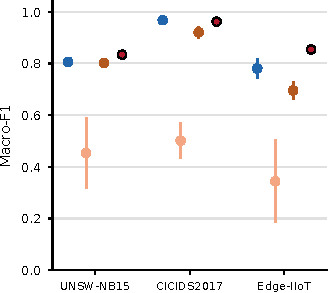
\includegraphics[width=0.3191\linewidth]{fig_main_results_a.pdf}\label{fig:mainresultsa}}\hfill%
\subfloat[False-alarm rate]{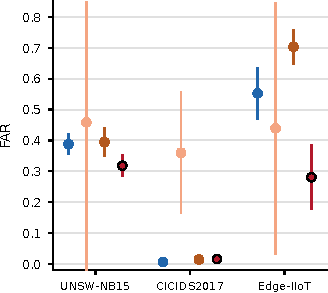
\includegraphics[width=0.3196\linewidth]{fig_main_results_b.pdf}\label{fig:mainresultsb}}\hfill%
\subfloat[Membership-inference audit]{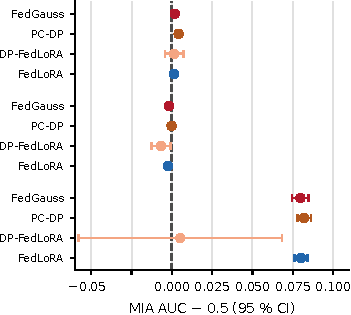
\includegraphics[width=0.3414\linewidth]{fig_main_results_c.pdf}\label{fig:mainresultsc}}
\\[4pt]

\includegraphics[width=0.5549\linewidth]{fig_main_results_legend.pdf}
\caption{Main results of \cref{tab:mainresults}, one question per
panel: (a) Macro-F1, (b) false-alarm rate (dots: method means;
whiskers: sample standard deviation over five seeds, three on
Edge-IIoT); (c) membership-inference audit AUC as deviation from
chance with 95\% confidence intervals.}
\label{fig:mainresults}
\end{figure*}
\par
\par
\begin{table}[pos=tbp]
\centering
\rmfamily
\small
\caption{Paired per-seed Macro-F1 differences (two-sided $95\%$ CIs;
\cref{sub:baselines}); $^{*}$ marks intervals that exclude zero.
``agg''/``pc'': aggregate vs.\ per-client release; ``naive''/``tight'':
basic-composition vs.\ zCDP accounting; ``98''/``full'': per-client release
dimension.}
\label{tab:cis}
\begin{tblr}
{
columns={co=-1},
cells={valign=m,halign=c},
columns={colsep=1pt},
rows={rowsep=2pt},
rows={ht=0pt},
stretch=0,
hline{1,Z}={wd=.08em},
hline{2}={wd=.05em},
cells={font=\fontsize{9pt}{8pt}},
row{1}={font=\bfseries\boldmath\fontsize{9pt}{8pt}},
row{even[2]}={bg=gray9!35},
}
Dataset & Contrast & Diff.\ [95\% CI] \\
UNSW & {\method\ (agg, $K=146$) $-$\\FedLoRA} & $+0.028$ [$+0.001$, $+0.055$]$^{*}$ \\
UNSW & {\method\ (agg, $K=146$) $-$\\FLTrust} & $+0.034$ [$+0.014$, $+0.054$]$^{*}$ \\
UNSW & {\method\ (agg, $K=146$) $-$\\PC-DP (tight)} & $+0.033$ [$-0.005$, $+0.070$] \\
UNSW & {\method\ (agg, $K=146$) $-$\\pc, 98} & $+0.086$ [$-0.039$, $+0.211$] \\
UNSW & {pc, 98 $-$\\pc, full (naive)} & $+0.295$ [$+0.033$, $+0.557$]$^{*}$ \\
CICIDS & {\method\ (agg, $K=146$) $-$\\FedLoRA} & $-0.003$ [$-0.022$, $+0.016$] \\
CICIDS & {\method\ (agg, $K=146$) $-$\\FLTrust} & $-0.012$ [$-0.024$, $+0.001$] \\
CICIDS & {\method\ (agg, $K=146$) $-$\\PC-DP (tight)} & $+0.042$ [$+0.014$, $+0.069$]$^{*}$ \\
CICIDS & {PC-DP (tight) $-$\\FedLoRA} & $-0.045$ [$-0.084$, $-0.005$]$^{*}$ \\
\end{tblr}
\end{table}
\par
\par
Paired per-seed statistics fix the strength of each claim at $n=5$
(\cref{tab:cis}; \cref{fig:basisb,fig:basisc}). The margin of \method\ over
DP-FedLoRA is large and consistent on both datasets. Against the non-private
and robust references the picture is dataset-dependent: the paired
differences over FedLoRA and FLTrust exclude zero on UNSW-NB15, supporting an
advantage there, whereas on CICIDS2017 \method\ is indistinguishable from
FedLoRA and marginally below FLTrust; \cref{app:fdrep} shows that this
proximity is sensitive to the evaluation split, while the private-versus-private
contrasts are preserved. Of the pre-specified set, five intervals exclude
zero: the UNSW-NB15 margins over both references and the per-client dimension
contrast, which confirms that the naive configuration is noise-dominated, and
on CICIDS2017 the aggregate-over-tightened margin and the tightened baseline
falling below FedLoRA. The aggregate-versus-tightened margins on UNSW-NB15
and the aggregate-versus-reference rows on CICIDS2017 do not exclude zero, so
no superiority is claimed there.
\par
\paragraph{Audit} Membership-inference audits show no measurable separation
between the DP release and the non-private reference on either benchmark
(\cref{fig:mainresultsc}). The full protocol and per-method detail are in
the Supplementary Material; the audit operates at sample level, whereas the
formal guarantee is client-level DP, and MIA AUC is an empirical check rather
than evidence for the formal bound.
\par
\subsection{Attribution and Ablation Experiments}
\label{sub:attribution}
\par
The main comparison varies the release boundary and the release dimension
together, so the two factors must be isolated. A matched factorial matrix
crosses the release boundary with the release dimension and the accounting
configuration at a fixed total budget. The recorded zCDP ledgers decompose
the joint accounting-and-clipping effect into its noise-scale factors:
replacing additive budget splitting with tight composition lowers the
calibrated per-coefficient noise by $4.4\times$ at equal total budget, and
basis-provenance and dimension sweeps isolate the representation factor. All
cells share the public checkpoint, partition, and seeds, and every leading
hyperparameter is selected on a validation split before any test evaluation.
The $K=98$ cells use a global-layout basis and the \method\ row the
validation-selected layerwise $K=146$ layout; cells are five-seed means
except the three-seed 98-coefficient public-basis row, and the naive
CICIDS2017 cell is an independent five-seed sample of the
\cref{tab:mainresults} naive configuration.
\par
\par
\begin{table*}[pos=tbp]
\centering
\rmfamily
\small
\caption{Matched release-boundary and dimension matrix, mean $\pm$ sample
standard deviation of accuracy and Macro-F1 at
$(\epsilon,\delta)=(8,10^{-5})$. The 98-random-basis row is
protocol-matched only on CICIDS2017 (\cref{tab:basisk}).}
\label{tab:matchedmatrix}
\begin{tblr}
{
columns={co=-1},
cells={valign=m,halign=c},
columns={colsep=4pt},
rows={rowsep=2pt},
rows={ht=0pt},
stretch=0,
hline{1,Z}={wd=.08em},
hline{3}={wd=.05em},
hline{2} = {3-4}{wd=.05em,rightpos=-.4,endpos=true},
hline{2} = {5-6}{wd=.05em,leftpos=-.4,endpos=true},
cells={font=\fontsize{9pt}{8pt}},
row{1}={font=\bfseries\boldmath\fontsize{9pt}{8pt}},
row{odd[3]}={bg=gray9!35},
cell{1}{3,5}={c=2}{},
}
& & UNSW-NB15 & & CICIDS2017 & \\
Release boundary & Dimension & Accuracy & Macro-F1 & Accuracy & Macro-F1 \\
Per-client Gaussian (naive) & full ambient update & 0.5483 $\pm$ 0.0728 & 0.4533 $\pm$ 0.1387 & 0.6108 $\pm$ 0.1016 & 0.5014 $\pm$ 0.0685 \\
Per-client Gaussian (tight) & 6{,}970 coefficients & 0.8165 $\pm$ 0.0142 & 0.8014 $\pm$ 0.0184 & 0.9524 $\pm$ 0.0119 & 0.9202 $\pm$ 0.0228 \\
Per-client Gaussian (tight) & 98 coefficients & 0.7735 $\pm$ 0.0787 & 0.7483 $\pm$ 0.1040 & 0.9718 $\pm$ 0.0074 & 0.9563 $\pm$ 0.0111 \\
Aggregate Gaussian & 6{,}970 coefficients & 0.6993 $\pm$ 0.1358 & 0.6581 $\pm$ 0.1770 & 0.9635 $\pm$ 0.0119 & 0.9406 $\pm$ 0.0205 \\
Aggregate Gaussian & 98, random basis & 0.8451 $\pm$ 0.0028 & 0.8364 $\pm$ 0.0033 & 0.9728 $\pm$ 0.0071 & 0.9568 $\pm$ 0.0116 \\
Aggregate Gaussian & 98, public basis & 0.8548 $\pm$ 0.0113 & 0.8484 $\pm$ 0.0132 & 0.9749 $\pm$ 0.0020 & 0.9608 $\pm$ 0.0028 \\
Aggregate Gaussian & layerwise 146 (\method) & 0.8430 $\pm$ 0.0103 & 0.8340 $\pm$ 0.0126 & 0.9758 $\pm$ 0.0022 & 0.9618 $\pm$ 0.0033 \\
\end{tblr}
\end{table*}
\par
\par
\begin{figure*}[pos=tbp]
\centering
\subfloat[Basis provenance (paired)]{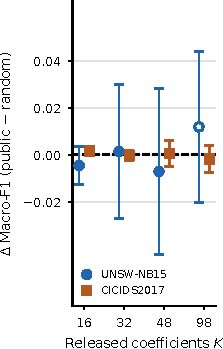
\includegraphics[width=0.2624\linewidth]{fig_attr_a.pdf}\label{fig:basisa}}\hfill%
\subfloat[UNSW-NB15]{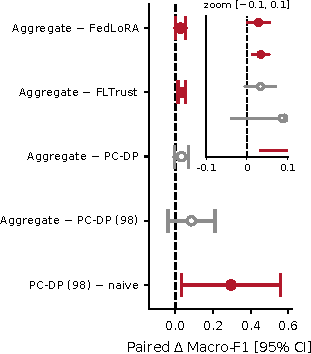
\includegraphics[width=0.3658\linewidth]{fig_attr_b.pdf}\label{fig:basisb}}\hfill%
\subfloat[CICIDS2017]{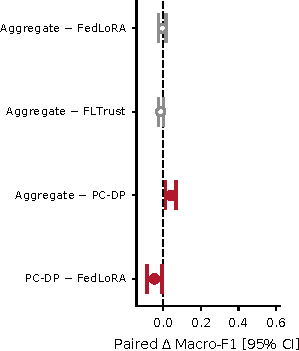
\includegraphics[width=0.3517\linewidth]{fig_attr_c.pdf}\label{fig:basisc}}
\caption{Attribution evidence under matched conditions. (a)~Basis
provenance as paired public $-$ random differences at each coefficient
budget (common three seeds; error bars: 95\% CI of the paired
difference); the hollow marker is the UNSW $K=98$ pair, whose
random-basis cell comes from the $\beta=0.98$ sweep-anchor family
and is therefore not protocol-matched (\cref{tab:basisk}).
(b), (c)~Paired Macro-F1 contrasts of \cref{tab:cis} on
UNSW-NB15 and CICIDS2017 (two-sided 95\% CIs; filled: the interval
excludes zero); the inset in (b) magnifies the near-zero region
$[-0.1, 0.1]$.}
\label{fig:basis}
\end{figure*}
\par
\paragraph{Matched factorial} Four observations follow from \cref{tab:matchedmatrix} and are
visualized in \cref{fig:matrixheatmap}. First, the naive-versus-tight
contrast within the per-client boundary shows that most of the reported
per-client collapse in the literature-style configuration is an accounting
and clipping artifact: with the zCDP ledger and a tuned clip, the
full-dimension per-client release recovers most of the collapse on both
benchmarks (\cref{tab:matchedmatrix}). Second, the headline margins over the
full-dimension per-client baseline (\cref{tab:cis}; \cref{fig:basis})
compare different release dimensions, so they mix the boundary with the
release dimension. At matched dimension the boundary effect is
dimension-dependent rather than stable: on UNSW-NB15 the matched-dimension difference changes sign between the
full-dimension pair, which favors the per-client branch, and the
98-coefficient pair, which favors the aggregate, and on CICIDS2017 the
matched pairs shrink to within noise. The release boundary
is therefore an operative lever jointly with the subspace release, not a
stable dimension-averaged effect. Third, the release dimension matters mainly
through the naive configuration and through the aggregate boundary; at
matched accounting the 98-coefficient and 146-coefficient releases sit
within roughly one standard deviation of each other. Fourth, and most
consequential for the design narrative, the seeded random orthonormal basis
performs within seed noise of the public-data basis in every protocol-matched
cell but one of \cref{tab:basisk}, and no matched public-basis advantage
is large enough to design for; the single unmatched cell, UNSW-NB15 at
$K=98$, is annotated in the table; \cref{fig:basisa} plots the paired
public-minus-random differences at every dimension. We therefore retract any design claim
that the public-data basis is a load-bearing component of \method: the operative
factors are the release boundary and the accounting configuration. The
public basis remains a reasonable default because it is available in the
evaluated setting at no extra cost, and the layerwise layout guards the
classifier head against a globally greedy allocation; neither effect is
measurable in utility at this scale.
\par
\begin{figure*}[pos=tbp]
\centering
\subfloat[UNSW-NB15]{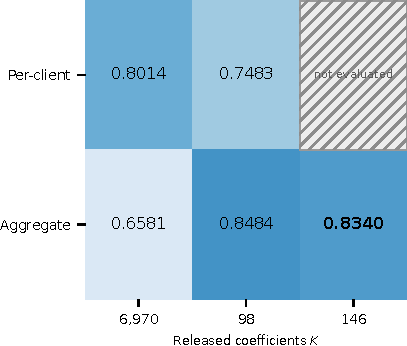
\includegraphics[width=0.4900\linewidth]{fig_matrix_heatmap_a.pdf}\label{fig:matrixheatmapa}}\hfill%
\subfloat[CICIDS2017]{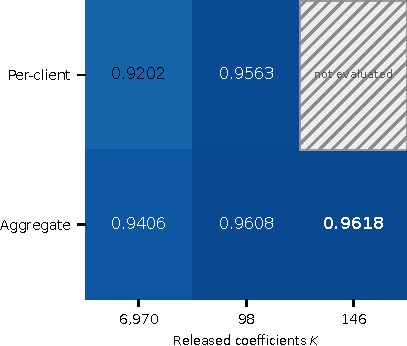
\includegraphics[width=0.4900\linewidth]{fig_matrix_heatmap_b.pdf}\label{fig:matrixheatmapb}}
\caption{Interaction heatmap of the matched factorial matrix
(\cref{tab:matchedmatrix}): Macro-F1 for the per-client and
aggregate boundaries across release dimensions; the hatched cell
marks the unevaluated per-client 146-coefficient configuration.}
\label{fig:matrixheatmap}
\end{figure*}
\par
\par
\begin{table}[pos=tbp]
\centering
\rmfamily
\small
\caption{Basis-provenance sweep: Macro-F1 mean over seeds $\{7,17,27\}$,
public-SVD versus seeded random orthonormal basis, validation-selected
protocol ($\beta=0$, $C=0.05$). Differences are within seed noise at
every dimension except CICIDS2017 $K=16$ ($+0.0016$). One cell is not
protocol-matched: no $\beta=0$ random-basis run exists at UNSW-NB15
$K=98$, so that cell reports the $\beta=0.98$ five-seed sweep-anchor
family ($0.8364\pm 0.0033$).}
\label{tab:basisk}
\begin{tblr}
{
columns={co=-1},
cells={valign=m,halign=c},
columns={colsep=6pt},
rows={rowsep=2pt},
rows={ht=0pt},
stretch=0,
hline{1,Z}={wd=.08em},
hline{2}={wd=.05em},
cells={font=\fontsize{9pt}{8pt}},
row{1}={font=\bfseries\boldmath\fontsize{9pt}{8pt}},
row{even[2]}={bg=gray9!35},
}
& $K=16$ & $K=32$ & $K=48$ & $K=98$\\
UNSW public & 0.8350 & 0.8422 & 0.8326 & 0.8484\\
UNSW random & 0.8395 & 0.8407 & 0.8396 & 0.8364\\
CICIDS public & 0.9640 & 0.9634 & 0.9638 & 0.9608\\
CICIDS random & 0.9623 & 0.9636 & 0.9632 & 0.9568\\
\end{tblr}
\end{table}
\par
\par
\paragraph{Trainable parameterization}
Two non-private controls run under the identical protocol, partition, and
public checkpoint: head-only, where LoRA factors are frozen and only the
classifier head trains and is aggregated, and full fine-tuning, where all
backbone parameters train. At this model scale the three
parameterizations sit within about one standard deviation of one another on
UNSW-NB15 and within 0.01 Macro-F1 on CICIDS2017 under the standard split
(\cref{tab:mainresults}). LoRA's role here is not
utility superiority but the definition of a compact, low-dimensional
trainable state that the subspace release can protect and communicate. The
DP aggregate release then exceeds all three non-private parameterizations on
UNSW-NB15, which we attribute to the clipping-regularization
effect documented below.
\par
\paragraph{Release ladder}
\par
\cref{tab:subspacemain} orders the release systems of increasing trust
on the same partitions, with each adjacent pair of rungs differing in exactly
one mechanism; \cref{fig:ladder} visualizes how each rung of
\cref{tab:subspacemain} adds a trust requirement or a release
mechanism.
\par
\begin{figure}[pos=tbp]
\centering
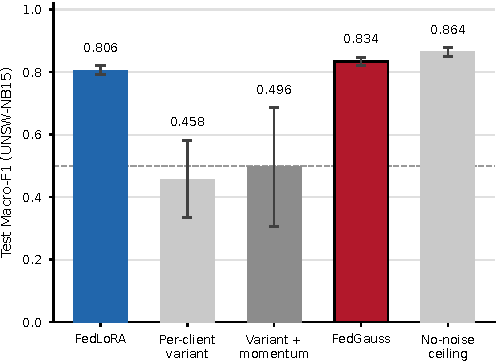
\includegraphics[width=\linewidth]{fig_ladder.pdf}
\caption{The release ladder of \cref{tab:subspacemain} on UNSW-NB15.}
\label{fig:ladder}
\end{figure}
\par
\par
\begin{table*}[pos=tbp]
\centering
\rmfamily
\small
\caption{Release-design study on UNSW-NB15 under the common protocol and
$(\epsilon,\delta)=(8,10^{-5})$; row labels give the seed count.}
\label{tab:subspacemain}
\begin{tblr}
{
columns={co=-1},
cells={valign=m,halign=c},
columns={colsep=4pt},
rows={rowsep=2pt},
rows={ht=0pt},
stretch=0,
hline{1,Z}={wd=.08em},
hline{2}={wd=.05em},
cells={font=\fontsize{9pt}{8pt}},
row{1}={font=\bfseries\boldmath\fontsize{9pt}{8pt}},
cell{Z}{1-Y}={font=\bfseries\boldmath\fontsize{9pt}{8pt}},
row{even[2]}={bg=gray9!35},
}
Release boundary & Method & Accuracy & Macro-F1 & FAR & MIA AUC\\
None (reference, $n=5$) & FedLoRA & 0.8207 $\pm$ 0.0103 & 0.8063 $\pm$ 0.0134 & 0.3883 $\pm$ 0.0340 & 0.5801 $\pm$ 0.0031\\
Per-client release ($n=3$) & DP-FedLoRA & 0.5325 $\pm$ 0.0515 & 0.4834 $\pm$ 0.0656 & 0.7466 $\pm$ 0.0889 & 0.5385 $\pm$ 0.0161\\
Per-client release ($n=3$) & {\method\\(per-client release)} & 0.4889 $\pm$ 0.1392 & 0.4576 $\pm$ 0.1235 & 0.5485 $\pm$ 0.3150 & 0.5255 $\pm$ 0.0401\\
Per-client release ($n=3$) & \method\ per-client + $\beta=0.9$, re-allocated $\epsilon$ & 0.5609 $\pm$ 0.1467 & 0.4965 $\pm$ 0.1896 & 0.5981 $\pm$ 0.3726 & 0.5277 $\pm$ 0.0351\\
{Projection only,\\no noise ($n=3$)} & Shared subspace + momentum & 0.8658 $\pm$ 0.0147 & 0.8643 $\pm$ 0.0139 & 0.1246 $\pm$ 0.0891 & 0.5468 $\pm$ 0.0210\\
Aggregate subspace ($n=5$) & {\method\\(zCDP, $\beta=0$, $K=146$)} & 0.8430 $\pm$ 0.0103 & 0.8340 $\pm$ 0.0126 & 0.3183 $\pm$ 0.0354 & 0.5797 $\pm$ 0.0042\\
\end{tblr}
\end{table*}
\par
\par
The release boundary is the main distinction between the two operating
regimes at a fixed budget: the aggregate subspace release attains the best
row, above the non-private FedLoRA reference. On CICIDS2017 the ordering is
conventional, with the private release just under the noiseless projection
ceiling. On UNSW-NB15 the ceiling ordering is regime-dependent: at the sweep
anchor ($K=98$, $\beta=0.98$) the private operating point lies marginally
above the noiseless projection, a regularization effect of coefficient
clipping at $C=0.05$ together with the projection, whereas the
validation-selected $\beta=0$ point sits below the same ceiling
(\cref{tab:subspacemain}). Projection and optimization ceilings, not
privacy noise, dominate the observed utility at this budget.
\par
\paragraph{Mechanism grid} \cref{tab:subspaceablation} isolates where the gain comes from by
varying the composition rule, server momentum, and coefficient clipping one
at a time around the aggregate release, and \cref{fig:exp3ablation}
visualizes both the absolute Macro-F1 of the recovery cells and each grid
cell's difference from the operating point. The grid is exploratory: the reported
operating point is the validation-selected configuration, not the best cell,
and no cell is bolded. The grid shows that tight accounting and calibrated
coefficient-space clipping explain most of the recovery, whereas the
contribution of momentum is dataset-dependent, and the direction holds
across all three seeds; because composition and clipping change together in
the basic-versus-zCDP contrast, this is evidence for their joint calibration
rather than an isolated zCDP effect.
\par
\begin{figure}[pos=tbp]
\centering
\subfloat[Accounting + clipping recovery ($\beta=0.9$)]{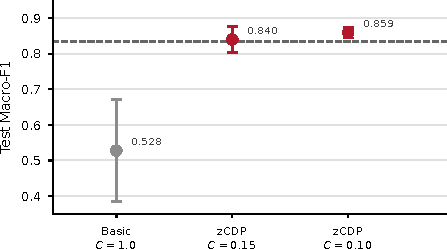
\includegraphics[width=0.8696\linewidth]{fig_mechanism_a.pdf}\label{fig:exp3ablationa}}\hfill%
\subfloat[Grid differences vs. validation-selected point]{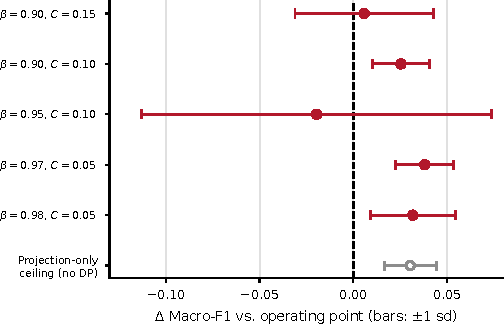
\includegraphics[width=0.9800\linewidth]{fig_mechanism_b.pdf}\label{fig:exp3ablationb}}
\caption{Mechanism grid of \cref{tab:subspaceablation} on UNSW-NB15
(three seeds). (a)~Absolute Macro-F1 (mean $\pm$ sd) under basic
composition and the two coarsest zCDP clips; the dashed line marks the
validation-selected operating point (a distinct configuration:
$\beta=0$, $C=0.05$, Macro-F1 $0.8340$). (b)~Grid differences
relative to that point (bars: $\pm$ 1~sd per cell); the hollow marker
is the conceptually distinct noiseless projection ceiling.}
\label{fig:exp3ablation}
\end{figure}
\par
\par
\par
\begin{table*}[pos=tbp]
\centering
\rmfamily
\small
\caption{Mechanism grid on UNSW-NB15 at $k_\ell=32$ ($K=98$), mean and
sample standard deviation over three seeds.}
\label{tab:subspaceablation}
\begin{tblr}
{
columns={co=-1},
cells={valign=m,halign=c},
columns={colsep=6pt},
rows={rowsep=2pt},
rows={ht=0pt},
stretch=0,
hline{1,Z}={wd=.08em},
hline{2}={wd=.05em},
cells={font=\fontsize{9pt}{8pt}},
row{1}={font=\bfseries\boldmath\fontsize{9pt}{8pt}},
row{even[2]}={bg=gray9!35},
}
Composition & Momentum $\beta$ & Coefficient clip & Accuracy & Macro-F1\\
Basic ($\epsilon/20$ per-round) & 0.9 & 1.0 & 0.5522 $\pm$ 0.1076 & 0.5276 $\pm$ 0.1436\\
zCDP & 0.9 & 0.15 & 0.8415 $\pm$ 0.0366 & 0.8397 $\pm$ 0.0368\\
zCDP & 0.9 & 0.10 & 0.8619 $\pm$ 0.0147 & 0.8593 $\pm$ 0.0152\\
zCDP & 0.95 & 0.10 & 0.8170 $\pm$ 0.0897 & 0.8144 $\pm$ 0.0934\\
zCDP & 0.97 & 0.05 & 0.8728 $\pm$ 0.0160 & 0.8720 $\pm$ 0.0155\\
zCDP & 0.98 & 0.05 & 0.8663 $\pm$ 0.0233 & 0.8657 $\pm$ 0.0228\\
\end{tblr}
\end{table*}
\par
The same one-factor grid on CICIDS2017 confirms the hierarchy with one
reversal: momentum is dataset-dependent, with $\beta\in\{0,0.98\}$
yielding a higher mean without the averaging window, because the data-rich
regime already converges within the schedule. CICIDS2017 therefore uses
$\beta=0$ in the main configuration.
\par
Crossing the release design, no-DP projection only versus the full aggregate
release at $\epsilon=8$, with and without server momentum, yields two
conclusions. First, the projection-plus-clipping representation accounts for
the bulk of the recovery over per-client release on both datasets:
projection with coefficient-space clipping and zCDP composition, without
momentum, already restores most utility. Second, momentum is a broad utility
lever whose sign is regime-dependent, adding about $+0.04$ in the small-data,
noise-dominated regime but harmful in the data-rich regime. This confirms it
as budget-free post-processing to be tuned per deployment rather than a
DP-specific repair.
\par
\paragraph{Anomaly-aware weighting}
Under matched noise, which keeps the uniform-calibrated noise scale,
anomaly-aware weighting is indistinguishable from uniform weights on both
datasets. Under the conservative realized-weight audit, which calibrates to
$\Delta = 2C\max_i w_i$ and is the price of keeping a per-round audit trail
for data-dependent weights, it degrades severely on UNSW-NB15, with one seed
collapsing, and mildly on CICIDS2017. The extension therefore buys
no measurable utility on either benchmark while forfeiting the formal
guarantee, which is why fixed uniform weights remain the default and
formally analyzed configuration. The influence-suppression theorem in the
supplementary material quantifies when such weights would matter: they suppress influence only when anomaly margins
are large, which the evaluated attacks do not create.
\par
\paragraph{Release dimension}
A per-tensor sweep $k_\ell\in\{8,16,32,64\}$ on UNSW-NB15 over three seeds
peaks at $k_\ell=32$: shrinking the subspace starves the projection of
capacity, and enlarging it spreads the release noise over more coefficients.
The basis-provenance sweep of \cref{tab:basisk} additionally shows
that, at matched accounting, dimension changes between $K=16$ and $K=98$
move Macro-F1 by at most $0.016$, so the dimension effect is far smaller
than the accounting effect once tight composition is in place. Enlarging the
subspace beyond 32 dimensions per tensor, doubling local epochs or the
learning rate, or extending the protocol to 30 or 40 rounds did not improve
the three-seed mean, which is capped by the noiseless projection ceiling of
each partition.
\par
Implementation-aligned ablations of the per-client release are reported in
\cref{app:ablations}, and \cref{fig:ablationfinal} visualizes the
utility ablations; the rank projection trades utility-neutral
behavior against a $61\times$ to $71\times$ raw-payload reduction.
\par
\subsection{Boundary and Sensitivity Analysis}
\label{sub:boundaries}
\par
This section varies the privacy budget, client heterogeneity, and LoRA rank
while fixing the remaining protocol, with three seeds per condition. The
sweeps use the sweep-anchor configuration specified in
\cref{tab:branchconfigs}, whereas the main results use the
validation-selected operating point; full configurations and values are
reported in \cref{tab:boundaries}.
\par
\par
\begin{table}[pos=tbp]
\centering
\rmfamily
\small
\caption{Full boundary sweeps, Macro-F1 mean over seeds $\{7,17,27\}$. The
$\alpha=0.5$ and $\epsilon=8$ cells are the three-seed counterparts of
the main-table configurations; the per-client budget sweep runs on
UNSW-NB15 only.}
\label{tab:boundaries}
\begin{tblr}
{
columns={co=-1},
cells={valign=m,halign=c},
columns={colsep=1pt},
rows={rowsep=2pt},
rows={ht=0pt},
stretch=0,
hline{1,Z}={wd=.08em},
hline{2,3,8,9,15,16}={wd=.05em},
hline{6,12}={wd=.05em},
cells={font=\fontsize{9pt}{8pt}},
row{1}={font=\bfseries\boldmath\fontsize{9pt}{8pt}},
cell{3,5,7,9,11,13,16,18}{2-Z}={bg=gray9!35},
cell{1}{3}={c=4}{},
cell{2,8,15}{1}={c=6}{halign=l},
cell{3,9,12}{1}={r=3}{},
cell{6}{1}={r=2}{},
}
& & sweep values & & & \\
\emph{Budget: $\epsilon=2\,/\,4\,/\,8\,/\,16$} & & & & & \\
UNSW & DP-FedLoRA & 0.3804 & 0.3903 & 0.4834 & 0.7104 \\
& \method\ (per-client) & 0.3783 & 0.4632 & 0.4576 & 0.4088 \\
& \method\ (aggregate) & 0.6132 & 0.6945 & 0.8622 & 0.8461 \\
CICIDS & DP-FedLoRA & 0.2695 & 0.2922 & 0.4946 & 0.4946 \\
& \method\ (aggregate) & 0.9295 & 0.9609 & 0.9634 & 0.9633 \\
\emph{Heterogeneity: $\alpha=0.1\,/\,0.5\,/\,1.0$} & & & & & \\
UNSW & FedLoRA & 0.8466 & 0.8048 & 0.8068 & -- \\
& DP-FedLoRA & 0.3848 & 0.4834 & 0.3870 & -- \\
& \method\ (aggregate) & 0.8240 & 0.8622 & 0.8213 & -- \\
CICIDS & FedLoRA & 0.8378 & 0.9613 & 0.9683 & -- \\
& DP-FedLoRA & 0.2614 & 0.4946 & 0.4550 & -- \\
& \method\ (aggregate) & 0.9601 & 0.9634 & 0.9645 & -- \\
\emph{Rank, CICIDS2017: $r=2\,/\,4\,/\,8\,/\,16$} & & & & & \\
& FedLoRA & 0.9597 & 0.9603 & 0.9613 & 0.9602 \\
& DP-FedLoRA & 0.2560 & 0.2892 & 0.4946 & 0.3407 \\
& \method\ (aggregate) & 0.9637 & 0.9611 & 0.9634 & 0.9629 \\
\end{tblr}
\end{table}
\par
\par
\paragraph{Privacy budget} \cref{tab:boundaries} reports the full sweeps. On UNSW-NB15 the
per-client curves are non-monotone: DP-FedLoRA improves only at the largest
tested budget, and the per-client release of \method\ peaks at moderate
budgets and reverses at the largest, because at larger total budgets the
fixed per-upload cap admits more noisy releases rather than reducing the
noise of each release. The aggregate release, whose noise follows joint
composition over the fixed protocol schedule, already leads the tested
per-client points at moderate budgets. On CICIDS2017 the identical
DP-FedLoRA values at the two largest budgets are a saturation effect of the
cap-implied total, while the aggregate curve saturates near the non-private
reference already at moderate budgets, and the residual low-budget gap
narrows as local training amortizes the release noise. These trends are empirical privacy and utility boundaries
rather than universal guarantees.
\par
\paragraph{Data heterogeneity} \cref{tab:boundaries} reports the Dirichlet sweep. FedLoRA is nearly
flat across $\alpha$ on both datasets. Per-client DP noise interacts
multiplicatively with skew: DP-FedLoRA is strongly sensitive, with a
seed spread that widens by an order of magnitude as skew increases, while
\method\ stays flat at a higher level with small spreads, and the modest
drop at the strongest skew on UNSW-NB15 suggests the basis stays aligned
under moderate skew. The aggregate release thus retains the level and the
stability of the non-private model on both datasets.
\par
\paragraph{Adapter rank} \cref{tab:boundaries} reports the rank sweep on CICIDS2017. The FedLoRA
and DP-FedLoRA payloads scale linearly with rank, while the aggregate release
transmits a constant-size release independent of rank
(\cref{tab:complexity}). Rank therefore interacts strongly with
per-client DP noise, whose utility stays low across ranks, and barely with
the aggregate release, which varies little within the tested range.
\par
\cref{fig:sensitivity} summarizes the three boundaries one factor at a
time: Macro-F1 versus privacy budget $\epsilon$ for the per-client DP family
and the aggregate release (panel a), versus Dirichlet $\alpha$ on CICIDS2017
(panel b), and versus LoRA rank on CICIDS2017 (panel c).
\par
\begin{figure*}[pos=tbp]
\centering
\subfloat[Privacy budget (UNSW-NB15)]{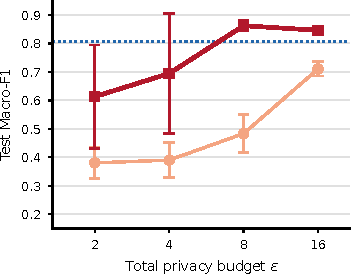
\includegraphics[width=0.3381\linewidth]{fig_sensitivity_a.pdf}\label{fig:sensitivitya}}\hfill%
\subfloat[Data heterogeneity (CICIDS2017)]{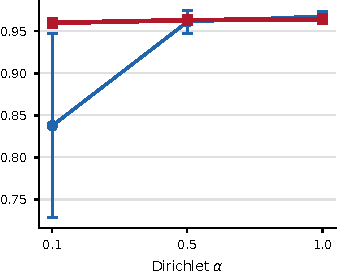
\includegraphics[width=0.3250\linewidth]{fig_sensitivity_b.pdf}\label{fig:sensitivityb}}\hfill%
\subfloat[LoRA rank (CICIDS2017)]{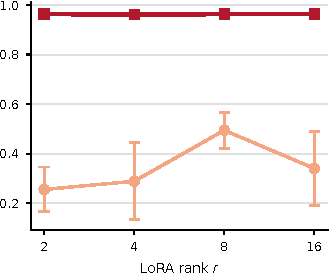
\includegraphics[width=0.3170\linewidth]{fig_sensitivity_c.pdf}\label{fig:sensitivityc}}
\\[4pt]

\includegraphics[width=0.4521\linewidth]{fig_sensitivity_legend.pdf}
\caption{Boundary and sensitivity analysis, one factor per panel
(three-seed means $\pm$ sample standard deviation): (a) privacy budget
$\epsilon$ on UNSW-NB15, whose aggregate series uses the $K=98$,
$\beta=0.98$ sweep-anchor family and whose dotted line marks the
non-private FedLoRA reference; (b) Dirichlet $\alpha$ on
CICIDS2017; (c) LoRA rank on CICIDS2017.}
\label{fig:sensitivity}
\end{figure*}
\par
These results support the stability of the validated configuration across
budgets, heterogeneity, and rank.
\par
\par
\subsection{Communication and Computational Cost}
\label{sub:scalability}
\par
This section scales the federation from 20 to 100 clients on CICIDS2017 and
varies the communication horizon from 10 to 30 rounds, keeping all other
protocol elements fixed. \cref{fig:comm} reports the per-round and
cumulative communication, \cref{fig:scalability} the protocol-length and
client-population effects, and \cref{fig:runtimemem} the measured
wall-clock and memory;
\cref{tab:complexity} lists the analytical and measured costs of the
main operating points. Across these operating points, the aggregate release
transmits a $40\times$ to $47\times$ smaller raw payload than the measured
per-client DP formats.
\par
\par
\begin{table*}[pos=tbp]
\centering
\rmfamily
\small
\caption{Analytical and measured costs of the main operating points.}
\label{tab:complexity}
\begin{tblr}
{
columns={co=-1},
cells={valign=m,halign=c},
columns={colsep=6pt},
rows={rowsep=2pt},
rows={ht=0pt},
stretch=0,
hline{1,Z}={wd=.08em},
hline{2}={wd=.05em},
cells={font=\fontsize{9pt}{8pt}},
row{1}={font=\bfseries\boldmath\fontsize{9pt}{8pt}},
row{even[2]}={bg=gray9!35},
}
Component & Cost model & CICIDS2017 & UNSW-NB15\\
FedLoRA payload & $4P_rM$ bytes & 239{,}760 B & 278{,}800 B\\
Per-client DP payload & $4P_rM$ bytes (active uploads) & 235{,}364 B & 273{,}689 B\\
\method\ payload & upstream $4KM$; released $4K$ & 5{,}840 B / 584 B & 5{,}840 B / 584 B\\
Full-model reference & $4P_fM$ bytes & 2{,}124{,}880 B & 3{,}374{,}160 B\\
Protection computation & $O(P_r)$ clip and sanitize; SVD projection; $O(KP_r)$ aggregate & -- & --\\
SecAgg overhead (analytical) & Bonawitz-style masking, $M=10$, $K=146$ & $\approx$1.19 kB & $\approx$1.19 kB\\
Measured resources & 20-round wall-clock; peak memory & 178.8 s, 46.7 MB & 18.0 s\\
\end{tblr}
\end{table*}
\par
\par
\paragraph{Client population} Within the tested client counts, \method\ changes little with population
size, because its release depends on the weighted aggregate rather than on
any single client, and its release size is independent of the federation
size (\cref{tab:complexity}).
\par
\paragraph{Protocol length and runtime} The protocol-length sweep shows the same stability from the convergence side
(\cref{tab:scalability} and \cref{fig:scalabilitya}): \method\ is
flat from 10 to 30 rounds, while FedLoRA first rises toward 20 rounds and
then degrades under the non-IID partitions. One CICIDS2017 federated run takes minutes and one UNSW-NB15 run under half
a minute on the reference workstation (\cref{tab:complexity};
\cref{fig:runtimemem}); these timings are simulator measurements and
exclude network delay, packet loss, client dropout, and production
secure-aggregation overhead.
\par
\par
\begin{table}[pos=tbp]
\centering
\rmfamily
\small
\caption{Client-count and protocol-length scalability on CICIDS2017 (three
seeds, original scaling campaign; Macro-F1 only in the rounds block).}
\label{tab:scalability}
\begin{tblr}
{
columns={co=-1},
cells={valign=m,halign=c},
columns={colsep=0pt},
rows={rowsep=2pt},
rows={ht=0pt},
stretch=0,
hline{1,Z}={wd=.08em},
hline{2,4,6,8,9}={wd=.05em},
cells={font=\fontsize{9pt}{8pt}},
row{1}={font=\bfseries\boldmath\fontsize{9pt}{8pt}},
row{2,4,6,9,11}={bg=gray9!35},
cell{8}{1}={c=4}{halign=l},
}
Clients & Method & Accuracy & Macro-F1 \\
20 & FedLoRA & 0.9794 $\pm$ 0.0094 & 0.9665 $\pm$ 0.0166 \\
20 & \method\ (ours) & 0.9763 $\pm$ 0.0013 & 0.9626 $\pm$ 0.0022 \\
50 & FedLoRA & 0.9763 $\pm$ 0.0073 & 0.9613 $\pm$ 0.0134 \\
50 & \method\ (ours) & 0.9768 $\pm$ 0.0032 & 0.9634 $\pm$ 0.0054 \\
100 & FedLoRA & 0.9766 $\pm$ 0.0049 & 0.9621 $\pm$ 0.0092 \\
100 & \method\ (ours) & 0.9760 $\pm$ 0.0010 & 0.9623 $\pm$ 0.0020 \\
\emph{Protocol length, 50 clients (Macro-F1)} & & & \\
Rounds 10 & FedLoRA & -- & 0.9578 $\pm$ 0.0082 \\
Rounds 10 & \method\ (ours) & -- & 0.9632 $\pm$ 0.0011 \\
Rounds 30 & FedLoRA & -- & 0.9409 $\pm$ 0.0045 \\
Rounds 30 & \method\ (ours) & -- & 0.9635 $\pm$ 0.0044 \\
\end{tblr}
\end{table}
\par
\par
\begin{figure*}[pos=tbp]
\centering
\subfloat[Per-round payload]{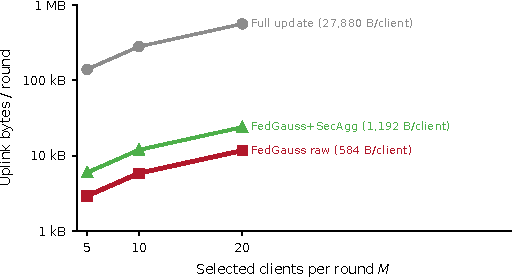
\includegraphics[width=0.4838\linewidth]{fig_comm_a.pdf}\label{fig:comma}}\hfill%
\subfloat[Cumulative volume ($M=10$)]{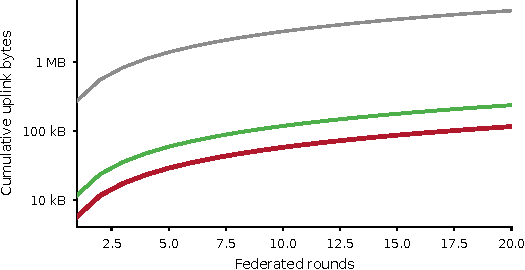
\includegraphics[width=0.4962\linewidth]{fig_comm_b.pdf}\label{fig:commb}}
\caption{Communication cost, one question per panel (analytical fp32
payloads): (a) uplink payload per round versus the round size $M$
(log scale), with SecAgg shown at its Bonawitz-style analytical
overhead; (b) cumulative uplink volume over a 20-round protocol at
$M=10$.}
\label{fig:comm}
\end{figure*}
\par
\begin{figure*}[pos=tbp]
\centering
\subfloat[Wall-clock time]{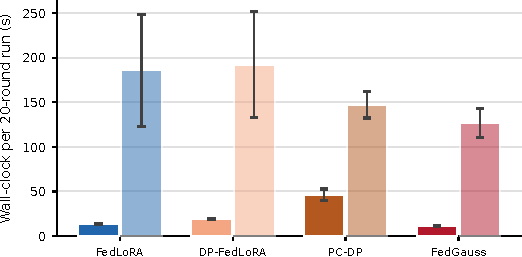
\includegraphics[width=0.4937\linewidth]{fig_runtime_memory_a.pdf}\label{fig:runtimemema}}\hfill%
\subfloat[Peak memory (CICIDS2017)]{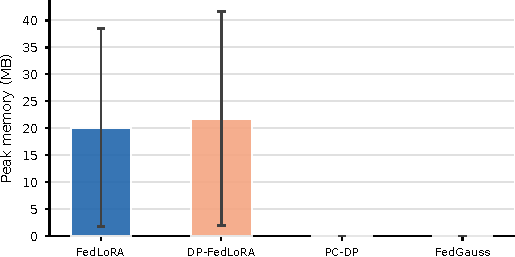
\includegraphics[width=0.4863\linewidth]{fig_runtime_memory_b.pdf}\label{fig:runtimememb}}
\\[4pt]

\includegraphics[width=0.2781\linewidth]{fig_runtime_memory_legend.pdf}
\caption{Measured cost of a 20-round run (five seeds): (a) wall-clock
time on the reference workstation; (b) peak memory on CICIDS2017
(UNSW-NB15 runs are CPU-only and report no GPU memory).}
\label{fig:runtimemem}
\end{figure*}
\par
\begin{figure*}[pos=tbp]
\centering
\subfloat[Protocol length (CICIDS2017)]{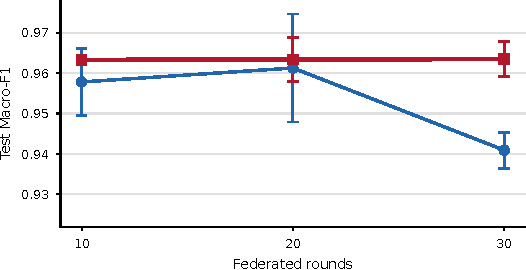
\includegraphics[width=0.4966\linewidth]{fig_scalability_a.pdf}\label{fig:scalabilitya}}\hfill%
\subfloat[Client population (CICIDS2017)]{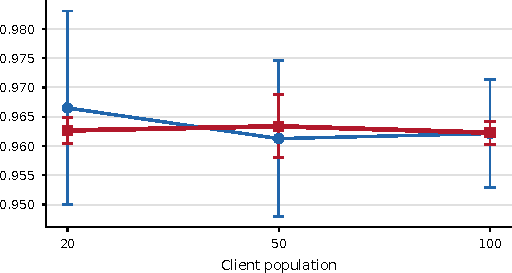
\includegraphics[width=0.4834\linewidth]{fig_scalability_b.pdf}\label{fig:scalabilityb}}
\\[4pt]

\includegraphics[width=0.2891\linewidth]{fig_scalability_legend.pdf}
\caption{Scalability on CICIDS2017, one factor per panel (three-seed
means $\pm$ sample standard deviation): (a) protocol length;
(b) client population.}
\label{fig:scalability}
\end{figure*}
\par
These results support the deployment stability of \method\ across client
populations and protocol lengths.
\par
\subsection{Robustness under Malicious Clients}
\label{sub:robustness}
\par
\paragraph{Stress-test configuration} Malicious clients use sign-flip, model-replacement, rank-collapse, or
subspace-shift updates with attack scale 5, and the malicious-client ratio
varies over 0.1, 0.2, and 0.3; each condition uses three seeds and is
reported as attack-condition means rather than clean-task operating points;
these are controlled stress tests under the evaluated attack families.
\par
Under these attacks, \method\ attains the highest attack-condition mean
Macro-F1 among the evaluated methods on UNSW-NB15, and its per-condition
values vary little across attack types and datasets; FLTrust is the most
attack-stable baseline in the evaluated per-condition results on both
datasets. Coefficient clipping, uniform aggregation, and the projection
jointly limit the effect of any single upload. This is
empirical stress evidence under the evaluated attack families rather than a
Byzantine-robustness guarantee; \cref{fig:robusta} tracks the mean
Macro-F1 as the malicious share grows, and \cref{fig:robustb} shows
the per-attack-type breakdown for the UNSW-NB15 methods.
\par
\begin{figure*}[pos=tbp]
\centering
\subfloat[Overall ratio effect]{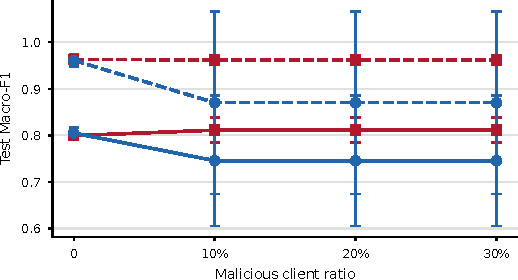
\includegraphics[width=0.4898\linewidth]{fig_robust_a.pdf}\label{fig:robusta}}\hfill%
\subfloat[Per-attack type: 10\% malicious (UNSW-NB15)]{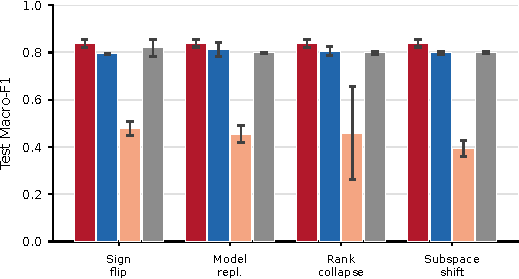
\includegraphics[width=0.4902\linewidth]{fig_robust_b.pdf}\label{fig:robustb}}
\\[4pt]

\includegraphics[width=0.5715\linewidth]{fig_robust_legend.pdf}
\caption{Robustness under malicious clients, one question per panel
(three seeds): (a) mean Macro-F1 as the malicious share grows, per
dataset and method, where each ratio averages the four attack
families, ratio zero is the clean reference of the same campaign,
and the UNSW-NB15 \MethodinCaption\ arm uses FLTrust aggregation;
(b) per-attack-type Macro-F1 at 10\% malicious clients on
UNSW-NB15.}
\label{fig:robust}
\end{figure*}
\par
\section{Discussion and Conclusion}
\label{sec:conclusion}
\par
\subsection{Practical Guidance}
\label{subsec:guidance}
\par
Two readings that would weaken the attribution are ruled out by controls
inside the evaluation: a dimension-or-clipping-interaction reading, ruled out
by the clip-matched cells of the release-boundary matrix, which leave the
aggregate margin positive only within the subspace
(\cref{sub:attribution}); and a regularization reading, bounded by
the noiseless projection ceilings that the private operating points attain on
both datasets (\cref{sub:attribution}). For deployment, the branch
follows the trust condition. Without a trusted aggregation boundary, the
per-client branch under the zCDP ledger and a tuned clip retains most
utility, with a modest utility gap relative to the aggregate release
(\cref{sub:attribution}). With a trusted service, or with secure aggregation and
client-side noise shares at an identical output distribution, the aggregate
branch with the subspace release recovers that margin, and the basis
provenance is a free choice.
\par
\subsection{Limitations}
\label{subsec:limitations}
\par
The formal guarantees apply to the stated release boundaries and client-level
adjacency. They do not solve all security problems in edge federated
learning. The current \texttt{secure} mode is a distributed-noise simulation
rather than a production cryptographic secure aggregation implementation.
The reported communication values are raw model payloads and exclude network
delay, packet loss, client dropout, protocol headers, cryptographic framing,
key exchange, and dropout recovery. The client partition is a controlled
Dirichlet construction and does not establish performance under natural
cross-site, cross-device, or temporal heterogeneity. On CICIDS2017 the split
is stratified random at record level and does not guarantee flow-disjoint or
time-ordered separation, so absolute numbers on that benchmark are internally
comparable only; \cref{app:fdrep} quantifies the duplicate overlap
and replicates the study on a duplicate-group-disjoint split
(\cref{sub:setup}). The attack pilots provide empirical stress
evidence rather than a universal robustness guarantee and do not include
targeted backdoor or adaptive detector-aware attacks. These boundaries limit
the deployment interpretation of the results.
\par
The evaluated design also reuses one stratified public proxy four times: backbone pre-training, subspace-basis
construction, the FLTrust root update, and feature-standardizer fitting. The
matched random-basis control (\cref{sub:attribution}) shows that
\method\ gains no utility advantage from the learned basis relative to a
seeded random basis of equal dimension, so the reuse creates no evidence of
structural advantage in the reported numbers. Deployment, however, still
requires access to a labeled public proxy that is representative of the
deployment traffic distribution. In operational intrusion detection, attack
distributions drift quickly, and a stale public proxy would degrade the
pre-trained backbone, the FLTrust root, and any learned basis jointly.
Deployments should refresh the public split on a schedule tied to drift
monitoring, or fall back to a random basis, which the matched matrix shows
costs no measurable utility at the tested dimensions.
\par
All conclusions are established on compact tabular MLPs. The release-boundary and release-dimension mechanisms
(clipping, zCDP composition, subspace projection) are dimension-generic and
their analysis is architecture-independent, but the specific utility
operating points, the optimal clipping norm, and the useful subspace
dimension do not transfer mechanically to large pre-trained backbones.
Validation on at least one production-scale backbone remains future work.
\par
\subsection{Conclusion}
\par
This paper asked whether the apparent collapse of DP-protected federated
LoRA is the inherent price of differential privacy or a design artifact, and
answered the question with a matched factorial evaluation under a two-branch
release protocol on three intrusion-detection benchmarks. Three scoped
conclusions follow. First, most of the naive per-client collapse is an
accounting and clipping artifact: under the zCDP ledger and a tuned clip,
the same per-client release recovers most of the loss on both
benchmarks (\cref{tab:mainresults}). Second, the release boundary matters jointly with the
representation space: the aggregate subspace release exceeds the non-private
references on UNSW-NB15 and attains the best row with the lowest false-alarm
rate on the Edge-IIoT replication, while its margin over the tightened
per-client baseline is modest and dimension-dependent
(\cref{sub:attribution}). Third, basis provenance has no measurable
effect in any protocol-matched comparison across the tested release dimensions; the operative design levers are the
accounting configuration and the joint release-boundary and representation
choice, which together price the two trust conditions: boundary-freedom at a
utility cost, versus a trusted aggregation boundary, realizable in output
distribution by secure aggregation with client-side noise shares, that
recovers most of that margin. The decision rules of
\cref{subsec:guidance} operationalize these conclusions for
deployment under a given trust boundary. Under the stated privacy budget and
trusted-aggregation assumption, the aggregate release satisfies the reported
DP bound; it is not a local-DP guarantee against a server that observes every
upload, and the deployment boundaries of \cref{subsec:limitations}
apply throughout.
\par
\appendix
\renewcommand{\thetable}{\arabic{table}}
\renewcommand{\thefigure}{\arabic{figure}}
\par
\section{Per-Client Release Ablations}
\label{app:ablations}
\par
\begin{figure*}[pos=tbp]
\centering
\subfloat[CICIDS2017]{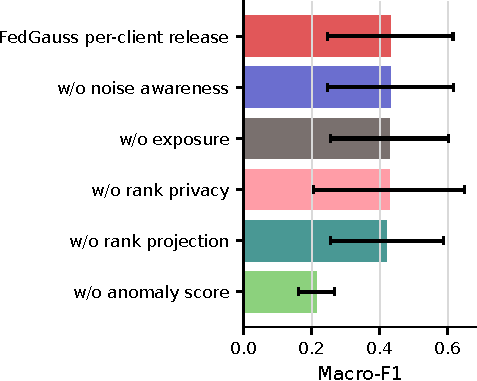
\includegraphics[width=0.5789\linewidth]{fig_paper_ablation_a.pdf}\label{fig:ablationfinala}}\hfill%
\subfloat[UNSW-NB15]{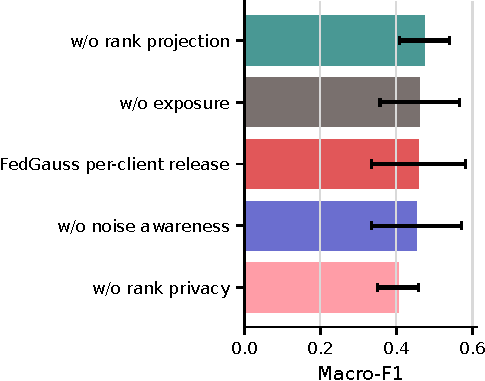
\includegraphics[width=0.4011\linewidth]{fig_paper_ablation_b.pdf}\label{fig:ablationfinalb}}
\caption{Utility ablations of the per-client release (UNSW-NB15 and
CICIDS2017, three seeds; components as in
\cref{tab:ablation}).}
\label{fig:ablationfinal}
\end{figure*}
\par
\par
\begin{table}[pos=tbp]
\centering
\rmfamily
\small
\caption{Implementation-aligned ablations of the per-client release of
\MethodinCaption.}
\label{tab:ablation}
\begin{tblr}
{
columns={co=-1},
cells={valign=m,halign=c},
columns={colsep=0pt},
rows={rowsep=2pt},
rows={ht=0pt},
stretch=0,
hline{1,Z}={wd=.08em},
hline{2}={wd=.05em},
cells={font=\fontsize{9pt}{8pt}},
row{1}={font=\bfseries\boldmath\fontsize{9pt}{8pt}},
row{even[2]}={bg=gray9!35},
}
Variant & {Rank-\\aware\\privacy} & {Noise-\\aware\\scoring} & {Exposure\\weighting} & {Evaluation\\purpose} \\
\method\ & Yes & Yes & Yes & {Full\\privacy-aware\\configuration} \\
{w/o\\rank\\privacy} & No & Yes & Yes & {Test\\rank-dependent\\noise control} \\
{w/o\\noise-aware\\scoring} & Yes & No & Yes & {Test\\anomaly\\calibration} \\
{w/o\\exposure\\weighting} & Yes & Yes & No & {Test\\contribution\\weighting} \\
{w/o\\anomaly\\scoring} & Yes & Yes & Yes & {Test\\anomaly-score\\contribution} \\
\end{tblr}
\end{table}
\par
\par
The ablations of \cref{tab:ablation}, visualized in
\cref{fig:ablationfinal}, show that the privacy-aware
components of the per-client release interact with the dataset. On UNSW-NB15
over three seeds, removing the rank-aware privacy allocation lowers mean
Macro-F1 from 0.4576 to 0.4047. Removing noise-aware scoring, a change of
$-0.004$, or exposure weighting, a change of $+0.004$, is neutral within one
standard deviation. Releasing the full parameter set without rank projection
raises utility to 0.4741, a change of $+0.017$, at the cost of a
substantially larger payload of approximately 3.28 MB per round.
\par
On CICIDS2017 over three seeds, the anomaly score is the load-bearing
component. Removing it collapses the per-client release from 0.4308 to
0.2138, while removing noise-aware scoring, exposure weighting, rank-aware
privacy, or the rank projection is neutral to mildly negative within the
large seed spread of this low-utility operating point.
\par
\section{Duplicate-Group-Disjoint Replication on CICIDS2017}
\label{app:fdrep}
\par
The standard CICIDS2017 split is stratified random at record level, so flows
with identical feature vectors can appear on both sides. Overall, $13.4\%$ of
test records ($28.6\%$ among attack records) share an exact 77-feature
duplicate with the training side. Because the released CSV variant omits flow
identifiers, an exact feature-vector group is the finest available flow
proxy. We therefore rebuilt the split at the group level. Duplicate groups
are assigned whole-side by stratified greedy allocation, and the per-class
test fractions remain exactly $0.200$. The split sizes change from
2{,}264{,}595/566{,}148 to 2{,}264{,}593/566{,}150, and the cross-side
duplicate count drops from 75{,}627 to zero. The backbone is re-trained on
the public fraction of the new training side (validation Macro-F1 0.983). The
four load-bearing CICIDS2017 families are then re-run over five seeds with
their configurations unchanged. This replication is a re-preparation: the
split, the public fraction, and the backbone change together. It therefore
measures the joint effect of removing duplicate overlap and re-composition,
not leakage removal alone.
\par
\cref{tab:fdrep} reports the result, and the reading we put on record is
a difference-in-differences one. The attribution contrasts are paired
comparisons within the same split, and all of them are preserved. The naive
collapse persists (0.3263 Macro-F1), and its recovery under tight accounting
persists (paired margin $+0.576$ [$+0.454$, $+0.699$] versus $+0.560$
[$+0.333$, $+0.786$] under the standard split). The headline margin of the
aggregate release over the tightened per-client baseline is preserved in
point estimate ($+0.046$ [$-0.006$, $+0.098$] versus $+0.042$ [$+0.014$,
$+0.069$] under the standard split), though the re-prepared interval now
includes zero. Absolute levels move with test-set composition: the
non-private reference strengthens to $0.9857\pm0.0022$ while the aggregate
release moves to $0.9487\pm0.0246$. Re-preparation also enlarges seed
variance itself, by roughly $7.4\times$ in standard deviation for the
aggregate release and $2.2\times$ for the tightened baseline. The mean shift
of the aggregate release is about $0.5$ of its own re-prepared standard
deviation, and three of the five seeds carry its direction consistently. We
report this split sensitivity and do not attribute it to a mechanism. The
consequence is adopted in the main text: proximity statements between the
aggregate release and the non-private references on CICIDS2017 are qualified
as standard-split results. Every private-versus-private contrast is a
within-split paired comparison and is preserved here.
\par
\par
\begin{table}[pos=tbp]
\centering
\rmfamily
\small
\caption{Duplicate-group-disjoint replication on CICIDS2017 (Macro-F1,
mean $\pm$ sample standard deviation, with paired 95\% CIs).}
\label{tab:fdrep}
\begin{tblr}
{
columns={co=-1},
cells={valign=m,halign=c},
columns={colsep=3pt},
rows={rowsep=2pt},
rows={ht=0pt},
stretch=0,
hline{1,Z}={wd=.08em},
hline{2,6,7}={wd=.05em},
cells={font=\fontsize{9pt}{8pt}},
row{1}={font=\bfseries\boldmath\fontsize{9pt}{8pt}},
row{2,4,7,9}={bg=gray9!35},
cell{6}{1}={c=3}{halign=l},
}
& Standard split & Group-disjoint \\
FedLoRA & 0.9649 $\pm$ 0.0137 & 0.9857 $\pm$ 0.0022 \\
DP-FedLoRA (naive) & 0.3608 $\pm$ 0.1658 & 0.3263 $\pm$ 0.1352 \\
PC-DP (tight) & 0.9202 $\pm$ 0.0228 & 0.9027 $\pm$ 0.0507 \\
\method\ (aggregate) & 0.9618 $\pm$ 0.0033 & 0.9487 $\pm$ 0.0246 \\
\emph{Paired contrasts} & & \\
{\method\ $-$\\PC-DP (tight)} & {$+0.042$\\{}[$+0.014$, $+0.069$]} & {$+0.046$\\{}[$-0.006$, $+0.098$]} \\
{PC-DP $-$\\naive} & {$+0.560$\\{}[$+0.333$, $+0.786$]} & {$+0.576$\\{}[$+0.454$, $+0.699$]} \\
{\method\ $-$\\FedLoRA} & {$-0.003$\\{}[$-0.022$, $+0.016$]} & {$-0.037$\\{}[$-0.067$, $-0.007$]} \\
\end{tblr}
\end{table}
\par
\par
\appendix
\section{Influence Suppression of the Anomaly-Weight Extension}
\label{app:influence}
This appendix analyzes the trusted-aggregator extension that replaces the
fixed uniform weights with anomaly-aware weights
(\cref{app:extensions}). The extension carries no DP claim;
\cref{thm:influence} characterizes only its robustness intuition, and
\cref{sec:evaluation} of the main paper reports its empirical cost.
\begin{theorem}[Influence suppression]\label{thm:influence}
Consider a malicious client $m$ and a benign client $b$ in the same round.
Define
\begin{equation}
\begin{aligned}
\Delta\rho_{mb}^t&=\hat{\rho}_m^t-\hat{\rho}_b^t,\\
\Delta a_{mb}^t&=a_m^t-a_b^t.
\end{aligned}
\end{equation}
Under the privacy- and anomaly-aware aggregation rule of \cref{subsec:anomaly-aggregation},
\begin{equation}
\begin{aligned}
\frac{w_m^t}{w_b^t}
&=
\frac{m_m}{m_b}
\exp\left(-\lambda_p\Delta\rho_{mb}^t-\lambda_a\Delta a_{mb}^t\right).
\end{aligned}
\end{equation}
Therefore, if $a_m^t-a_b^t\geq \Delta_a>0$ and the privacy-exposure terms are
equal, the malicious client's relative influence is suppressed by a factor
of at least $\exp(-\lambda_a\Delta_a)$, up to the data-size ratio.
\end{theorem}
\begin{proof}[Proof sketch]
The result follows directly by taking the ratio of the two aggregation
weights. The shared normalization denominator cancels out. A larger anomaly
margin or a larger $\lambda_a$ exponentially reduces the relative weight of
the suspicious adapter.
\end{proof}
The adapter anomaly score is not a cryptographic guarantee; it is a
robustness mechanism that reduces the influence of updates that deviate from
normal adapter-space behavior. Malicious LoRA updates often concentrate
attack power in a few low-rank directions. By combining subspace deviation,
protected-update magnitude, and rank-collapse indicators, \method\ penalizes
updates that are both structurally abnormal and potentially damaging. Because
the anomaly score is used in a soft aggregation weight rather than a hard
rejection rule, benign clients with non-IID data are not immediately
discarded.
\section{Trusted-Aggregator Extensions}
\label{app:extensions}
\subsection{History-Based Privacy Controller}
\label{subsec:controller}
For client $i$ at round $t$, the controller derives a risk score only from
previously released protected updates and the previous protected aggregate.
The current clean update is not inspected before the privacy parameters are
selected. The risk score is defined as
\begin{equation}
\mathcal{R}_i^t =
0.35\,\tilde{s}_i^{t-1}
+0.25\,\tilde{\kappa}_i^{t-1}
+0.20\,\tilde{d}_i^{t-1}
+0.20\,\tilde{c}_i^{t-1},
\end{equation}
where all terms are normalized to $[0,1]$ across the selected clients. The
historical sensitivity term is computed from the previously released
protected update,
\begin{equation}
s_i^{t-1}=\sum_{\ell\in\mathcal{L}}\|\widehat{\Delta W}_i^{\ell,t-1}\|_F,
\end{equation}
the spectral-concentration term is measured by
\begin{equation}
\kappa_i^{t-1}=
\frac{\sum_{\ell\in\mathcal{L}}\|\widehat{\Delta W}_i^{\ell,t-1}\|_2}
{\sum_{\ell\in\mathcal{L}}\|\widehat{\Delta W}_i^{\ell,t-1}\|_F+\xi}.
\end{equation}
The subspace-drift term compares the previous protected client update with
the previous protected aggregate, while the collapse term measures rank
concentration. Larger historical magnitude, concentration, drift, or
collapse leads to a more conservative privacy allocation. The controller is
therefore post-processing of earlier protected releases.
\par
The per-round privacy budget is assigned by
\begin{equation}
\epsilon_i^t =
\epsilon_{\min}
+
(\epsilon_{\max}-\epsilon_{\min})
\left(1-s(\gamma(\mathcal{R}_i^t-\tau_r))\right),
\end{equation}
where $s(x)=1/(1+\exp(-x))$, $\gamma$ controls the sharpness of the
controller, and $\tau_r$ is a risk threshold. High-risk clients therefore
receive smaller privacy budgets and stronger perturbation.
\subsection{Adapter Anomaly Scoring}
\label{subsec:anomaly-scoring}
The scoring mechanism in this subsection operates on \emph{individual}
protected uploads. It is therefore part of the per-client release, and it can
be attached to the aggregate release only in the trusted-aggregator
extension, in which the aggregation service does observe individual clipped
uploads; in the formally analyzed aggregate release configuration no anomaly
score is computed at all, because aggregation uses fixed uniform weights.
The server computes the score using only the protected upload, the current
global reference, and robust statistics accumulated from earlier protected
uploads. Since local perturbation changes update geometry, the score is
noise-aware; larger reported noise relaxes the thresholds.
\begin{equation}
\begin{aligned}
a_i^t =
&\frac{[d_{\mathrm{sub}}(\widetilde{\Delta W}_i^t,\Delta W_g^{t-1})-\tau_d(\sigma_{i,t})]_+}{1+\sigma_{i,t}}
\\
&+\frac{[n_i^t-\tau_s(\sigma_{i,t})]_+}{1+\sigma_{i,t}}
\\
&+c_{\mathrm{rank}}(\widehat{\Delta W}_i^t).
\end{aligned}
\end{equation}
where $[x]_+=\max(x,0)$. The three indicators are computed from the
protected LoRA matrices, using the notation $d_{\mathrm{sub}}$ for the
subspace deviation, $n_i^t$ for the update-magnitude score, and
$c_{\mathrm{rank}}$ for the rank-collapse indicator. The subspace deviation
compares the top-$r$ left singular subspace of the upload with that of the
current global reference state,
\begin{equation}
d_{\mathrm{sub}}(\widetilde{\Delta W}_i^t,\Delta W_g^{t-1})
=
\frac{1}{\sqrt{2}}\|U_i^t(U_i^t)^\top-U_g^{t-1}(U_g^{t-1})^\top\|_F .
\end{equation}
The update-magnitude score is the Euclidean norm of the flattened protected
adapter update,
\begin{equation}
n_i^t=\|\operatorname{vec}(\widetilde{u}_i^t)\|_2,
\end{equation}
and the rank-collapse indicator is
\begin{equation}
c_{\mathrm{rank}}(\widehat{\Delta W}_i^t)
=
\left[
1-
\frac{\sum_{k=1}^{r}\sigma_k(\widehat{\Delta W}_i^t)}
{r\sigma_1(\widehat{\Delta W}_i^t)+\xi}
\right]_+ .
\end{equation}
Here $\sigma_k(\cdot)$ denotes the $k$th singular value and $\xi$ is a small
stability constant. The noise-dependent thresholds $\tau_d(\hat{\sigma}_i^t)$
and $\tau_s(\hat{\sigma}_i^t)$ relax anomaly penalties when stronger privacy
noise is expected. In implementation, these thresholds can be estimated from
warm-up rounds or historical protected adapters using robust statistics, for
example
\begin{equation}
\tau_z(\hat{\sigma})=
\mathrm{median}(z)+\eta_z\mathrm{MAD}(z)+\beta_z\hat{\sigma},
\quad z\in\{d,s\},
\end{equation}
where $\mathrm{MAD}$ is the median absolute deviation and $\beta_z\hat{\sigma}$
compensates for privacy-induced variation. This design makes anomaly scoring
reproducible and prevents strongly perturbed benign adapters from being
treated as malicious solely because their spectra or subspaces are noisier.
These indicators are useful because malicious LoRA updates often exploit a
small number of high-impact directions rather than distributing changes
across the full parameter space.
\subsection{Privacy- and Anomaly-Aware Aggregation}
\label{subsec:anomaly-aggregation}
Let $\hat{\rho}_i^t$ denote the cumulative privacy exposure estimated from
coarse privacy-consumption buckets:
\begin{equation}
\hat{\rho}_i^t=
\min\left(1,\frac{\sum_{s=1}^t\hat{\epsilon}_i^s}{\epsilon_{\mathrm{total}}}\right).
\end{equation}
The aggregation weight is computed from sample count, cumulative exposure,
and anomaly score:
\begin{equation}
w_i^t =
\frac{
m_i\exp(-\lambda_p\hat{\rho}_i^t-\lambda_a a_i^t)
}{
\sum_j m_j\exp(-\lambda_p\hat{\rho}_j^t-\lambda_a a_j^t)
}.
\end{equation}
The server updates the global trainable state by
\begin{equation}
\widetilde{u}^{t}=\sum_i w_i^t\widetilde{u}_i^t .
\end{equation}
The server adds $\widetilde{u}^{t}$ to the current global state and
rank-projects the resulting LoRA matrices, while the head tensors are
unchanged by this projection. The weighting rule reduces the repeated
influence of clients with high privacy exposure and suppresses suspicious
adapter updates without requiring access to raw data or exact descriptors.
This weighting belongs to the per-client release and to the trusted-aggregator
extension; it is \emph{not} part of the formally analyzed aggregate-release
configuration, which uses fixed uniform weights. In the configurations where
weighting is enabled, $\lambda_p=0.5$, $\lambda_a=1.0$, and anomaly scoring
starts after three warm-up rounds.
\section{Full Proofs}
\label{app:proofs}
\begin{proof}[Proof of \cref{thm:perround} of the main paper]
Let $D$ and $D'$ be adjacent federated datasets differing in the complete
local dataset of client $i$. The clipped updates of all other clients are
identical functions of their unchanged data. Both $\bar u_i^t(D)$ and
$\bar u_i^t(D')$ have Euclidean norm at most $C$ by construction of the
clipping map, so $\|\bar u_i^t(D)-\bar u_i^t(D')\|_2\le 2C$; this bounds the
$\ell_2$ sensitivity of the released vector-valued function. The classical
Gaussian-mechanism bound \cite{dwork2014algorithmic} then yields
$(\epsilon_{i,t},\delta_{i,t})$-DP for the stated noise scale.
Post-processing immunity is the standard closure property of DP
\cite{dwork2014algorithmic}: any data-independent map applied to sanitized
outputs preserves the guarantee. The guarantee concerns sanitized releases,
not endpoint state or unprotected side channels.
\end{proof}
\begin{proof}[Proof of \cref{thm:perround} of the main paper (sequential composition)]
Fix any realized transcript prefix; under the per-client release, earlier
releases of the same client may have shifted its local state, but as in
\cref{prop:round} of the main paper the conditional sensitivity of the current
release is still bounded by $2C$, because the clipping map bounds the
released norm independently of the history. Each participating round then
releases one sanitized update for the client, and for any output set of the
joint transcript the standard sequential-composition argument
\cite{dwork2014algorithmic,abadi2016deep} multiplies the per-release
likelihood ratios along the transcript, which adds the $\epsilon$ terms and
the $\delta$ terms. Tighter accountants (for example, zCDP as used for the
aggregate release below) can be substituted without changing the release
mechanism.
\end{proof}
\begin{proof}[Proof of \cref{prop:round} of the main paper]
The global adapter state, the selected set $\mathcal{S}_t$, and each client
update in round $t$ are deterministic functions of the realized prefix
$h_{t-1}$ and the private data; conditioning on $h_{t-1}$ freezes all of
them. This is the standard device that makes adaptive multi-round accounting
sound: earlier releases change the optimization trajectory, but once the
trajectory prefix is fixed, the round-$t$ release is an ordinary Gaussian
mechanism. Let $D$ and $D'$ differ in the complete local dataset of client
$j\in\mathcal{S}_t(h_{t-1})$ (if $j\notin\mathcal{S}_t(h_{t-1})$ the two
conditional releases are identical and the claim is trivial). All
coefficients are clipped in coefficient space to norm at most $C$ regardless
of $h_{t-1}$, so $\|\bar c_j^t(D,h_{t-1})\|_2\le C$ and
$\|\bar c_j^t(D',h_{t-1})\|_2\le C$, and the two conditional aggregates
differ only in the $j$-th term:
\begin{equation}
\big\|g(D\mid h_{t-1})-g(D'\mid h_{t-1})\big\|_2\le
\tfrac{2C}{|\mathcal{S}_t(h_{t-1})|}=\Delta^t .
\end{equation}
The Gaussian mechanism is $\tfrac{\Delta^2}{2\sigma^2}$-zCDP for any function
of $\ell_2$ sensitivity at most $\Delta$ \cite{bun2016concentrated}.
Substituting $\sigma_t=\Delta^t/\sqrt{2\rho_r}$ gives exactly $\rho_r$-zCDP
conditionally on $h_{t-1}$. The bases $Q_\ell$ and the weights are
data-independent by the release model, so neither the projection nor the
weighting adds data dependence. Client selection depends only on the public
sampling rule and the realized prefix, not on private data, and dropouts
change $|\mathcal{S}_t(h_{t-1})|$ but not the conditional sensitivity
argument, because the clipping bound $C$ is history-free.
\end{proof}
\textbf{Remark (client dropout and noise-share consistency).}
\cref{prop:round} of the main paper conditions on the realized participation set,
which is all that dropout requires. A dropout before the round-$t$ release
changes $M_t=|\mathcal{S}_t(h_{t-1})|$ and with it $\Delta^t=2C/M_t$ and
$\sigma_t$; the per-round ledger stores exactly these realized values, so the
budget is re-derived from realized participation rather than from the planned
schedule. A client that releases nothing burns no budget, and the
participation cap counts uploads. The same conditioning keeps the noise-share
realization consistent. Because client selection depends only on the public
sampling rule and the realized prefix, $M_t$ is public to the contributors.
Each of the $M_t$ surviving clients can then draw an independent noise share
of variance $\sigma_t^2/M_t$ per coefficient, so the summed shares have
exactly the calibrated variance $\sigma_t^2I_K$. If an implementation
publishes only a bound $M_t\ge m_{\min}$, calibrating the summed noise to
$\sigma(m_{\min})=(2C/m_{\min})/\sqrt{2\rho_r}$ over-noises every realized
round by the factor $M_t/m_{\min}$ in standard deviation. The ledger then
charges the conservative scale. No guarantee beyond
Propositions~2 and~3 of the main paper is claimed. The remark
records that transcript-conditioned calibration and distributed noise shares
remain consistent under dropout.
\begin{proof}[Proof of \cref{prop:composition} of the main paper]
Each round-$t$ mechanism is $\rho_r$-zCDP conditionally on every realized
transcript prefix by \cref{prop:round} of the main paper. Adaptive zCDP composition
\cite{bun2016concentrated} therefore applies: because the conditional
guarantee holds for every prefix, the adaptive transcript
$(\mathcal{M}_1,\dots,\mathcal{M}_T)$, in which each round's mechanism and
participant set may depend on all earlier released aggregates, is jointly
$\sum_{t=1}^T\rho_r=T\rho_r=\rho$-zCDP. The conversion bound of
\cite{bun2016concentrated} states that $\rho$-zCDP implies
$(\rho+2\sqrt{\rho\ln(1/\delta)},\delta)$-DP for every $\delta>0$. Solving
$\rho+2\sqrt{\rho\ln(1/\delta)}\le\epsilon$ for $\rho$ yields precisely
$\rho\le\big(\sqrt{\ln(1/\delta)+\epsilon}-\sqrt{\ln(1/\delta)}\big)^2$,
which is the total zCDP budget $\rho$ of the main paper; hence the adaptive transcript satisfies the
target $(\epsilon,\delta)$. Because client sampling is public and the
client's data may influence every round's aggregate, composing all $T$
releases is conservative and covers arbitrary repeated participation; no
amplification is claimed.
\end{proof}
\begin{proof}[Proof of \cref{prop:composition} of the main paper (post-processing)]
zCDP is closed under post-processing \cite{bun2016concentrated}: if
$\mathcal{M}$ is $\rho$-zCDP and $g$ is any data-independent measurable map,
then $g\circ\mathcal{M}$ is $\rho$-zCDP. The decoding applies the fixed
public basis $\{Q_\ell\}$; the momentum recursion
$m^t=\beta m^{t-1}+(1-\beta)\tilde u^t$ is a deterministic linear map of the
transcript; and the controller and noise-aware thresholds of
\cref{app:extensions} read only previously released objects. All are
data-independent functions of the transcript, so the guarantee is unchanged
and no budget is consumed.
\end{proof}
\begin{algorithm}[tbp]
\caption{Per-client Gaussian release branch (baseline; no trusted aggregator)}
\label{alg:pcrelease}
\begin{algorithmic}[1]
\Require own update $u_i^t$; clip norm $C$; the representation space of
the configuration (Table~Table~7 of the main paper); per-client ledger
$\mathcal{Z}_i$ with its per-upload debit ($\rho_r$, or
$(\epsilon_{i,t},\delta_{i,t})$ for the naive baseline); cap $n_{\max}$
\State Skip the release if the cumulative ledger plus this debit would
exceed the client budget, or if $n_{\max}$ uploads have been released
\Comment{the check precedes the release}
\State Clip: $\bar u_i^t\gets u_i^t\min\{1,C/(\|u_i^t\|_2+10^{-12})\}$
\State Sensitivity $\Delta_c\gets 2C$ \Comment{replacement adjacency of
one own release}
\State $\sigma_{i,t}\gets$ calibrated by \cref{alg:zcdp} from the
per-client ledger
\State Upload $\widetilde u_i^t\gets\bar u_i^t+\mathcal{N}(0,\sigma_{i,t}^2 I)$
\Comment{sanitized on-device; the server receives only this noised update}
\State Append the debit to the client ledger
\State \Return $\widetilde u_i^t$ \Comment{aggregated by
Algorithm~Algorithm~1 of the main paper}
\end{algorithmic}
\end{algorithm}
\begin{algorithm}[tbp]
\caption{Privacy-budget allocation and ledger update}
\label{alg:zcdp}
\begin{algorithmic}[1]
\Require total $(\epsilon,\delta)$; planned releases $T$ (aggregate) or
per-client caps (per-client branch)
\State $\rho\gets\big(\sqrt{\ln(1/\delta)+\epsilon}-\sqrt{\ln(1/\delta)}\big)^2$
\State Aggregate branch: per-release zCDP cost $\rho_r\gets\rho/T$; per-round
noise $\sigma_t\gets\Delta^t/\sqrt{2\rho_r}$
\State Per-client branch: the per-upload noise $\sigma_{i,t}$ is fixed by
the configuration; each upload debits the zCDP cost
$\rho_r\gets\Delta_c^2/(2\sigma_{i,t}^2)$ at the replacement
sensitivity $\Delta_c\gets 2C$; a client's at most
$n_{\max}$ uploads zCDP-compose to at most $n_{\max}\rho_r\le\rho$,
converted once to $(\epsilon_c\le\epsilon,\delta)$
\State Per-client baseline (naive): per-upload $(\epsilon_r,\delta_r)$
under basic composition (\cref{thm:perround} of the main paper); the cap
composes at most $(n_{\max}\epsilon_r,\,n_{\max}\delta_r)$
\State Each round: append the spent debit (aggregate: $\rho_r$; per-client:
the uploading client's cost); a participant whose cumulative cost would
exceed the total, or whose upload count would reach $n_{\max}$, is
excluded from selection
\State Post-processing (decode, momentum, evaluation) spends nothing
\Comment{\cref{prop:composition} of the main paper}
\State \Return branch ledgers; the noise scales $\sigma_t$ and
$\sigma_{i,t}$
\end{algorithmic}
\end{algorithm}
\section{Per-Client Release and Budget-Ledger Algorithms}
\label{app:algs}
This appendix reproduces the per-client release procedure and the
privacy-budget allocation for reference; the main paper states the same
rules in prose in its \cref{sec:analysis}.
\bibliographystyle{elsarticle-num}
\bibliography{reference}
\end{document}
